%% The "\appendix" call has already been made in the declaration
%% of the "appendices" environment (see thesis.tex)
\chapter{Auxiliary Plots}

\section{Pre-Fit modelling}
\label{app:pre-fit_di-lepton}
For the di-lepton channel, the background composition is shown in Figure~\ref{fig:2l_region_comp}. The same general pattern is observed, with the $t\bar{t}+$light and $t\bar{t}+\geq 2b$ regions exhibiting high purity. Here, the $t\bar{t}+\geq 1c$ process is more cleanly separated than in the single lepton case, benefiting from the additional constraints of the di-lepton final state. As in the single lepton channel, the $t\bar{t}+\geq 2b$ background remains the dominant contribution in the signal regions, with $t\bar{t}+1b$ and other processes becoming more relevant in the low- and high-$p_{T}^{H}$ bins, respectively.\\
\\
For the di-lepton channel, five control regions are used, as illustrated in Figure~\ref{fig:2l_data_mc_pre_fit_CR}. Again, the ratio of data to MC predictions indicates a very good level of pre-fit agreement within the defined uncertainties. The six resolved signal regions are shown in Figure~\ref{fig:2l_data_mc_pre_fit_SR}, with similarly strong pre-fit agreement. No boosted signal region is defined in the di-lepton channel due to limited statistics.
\begin{figure}[H]
    \centering
    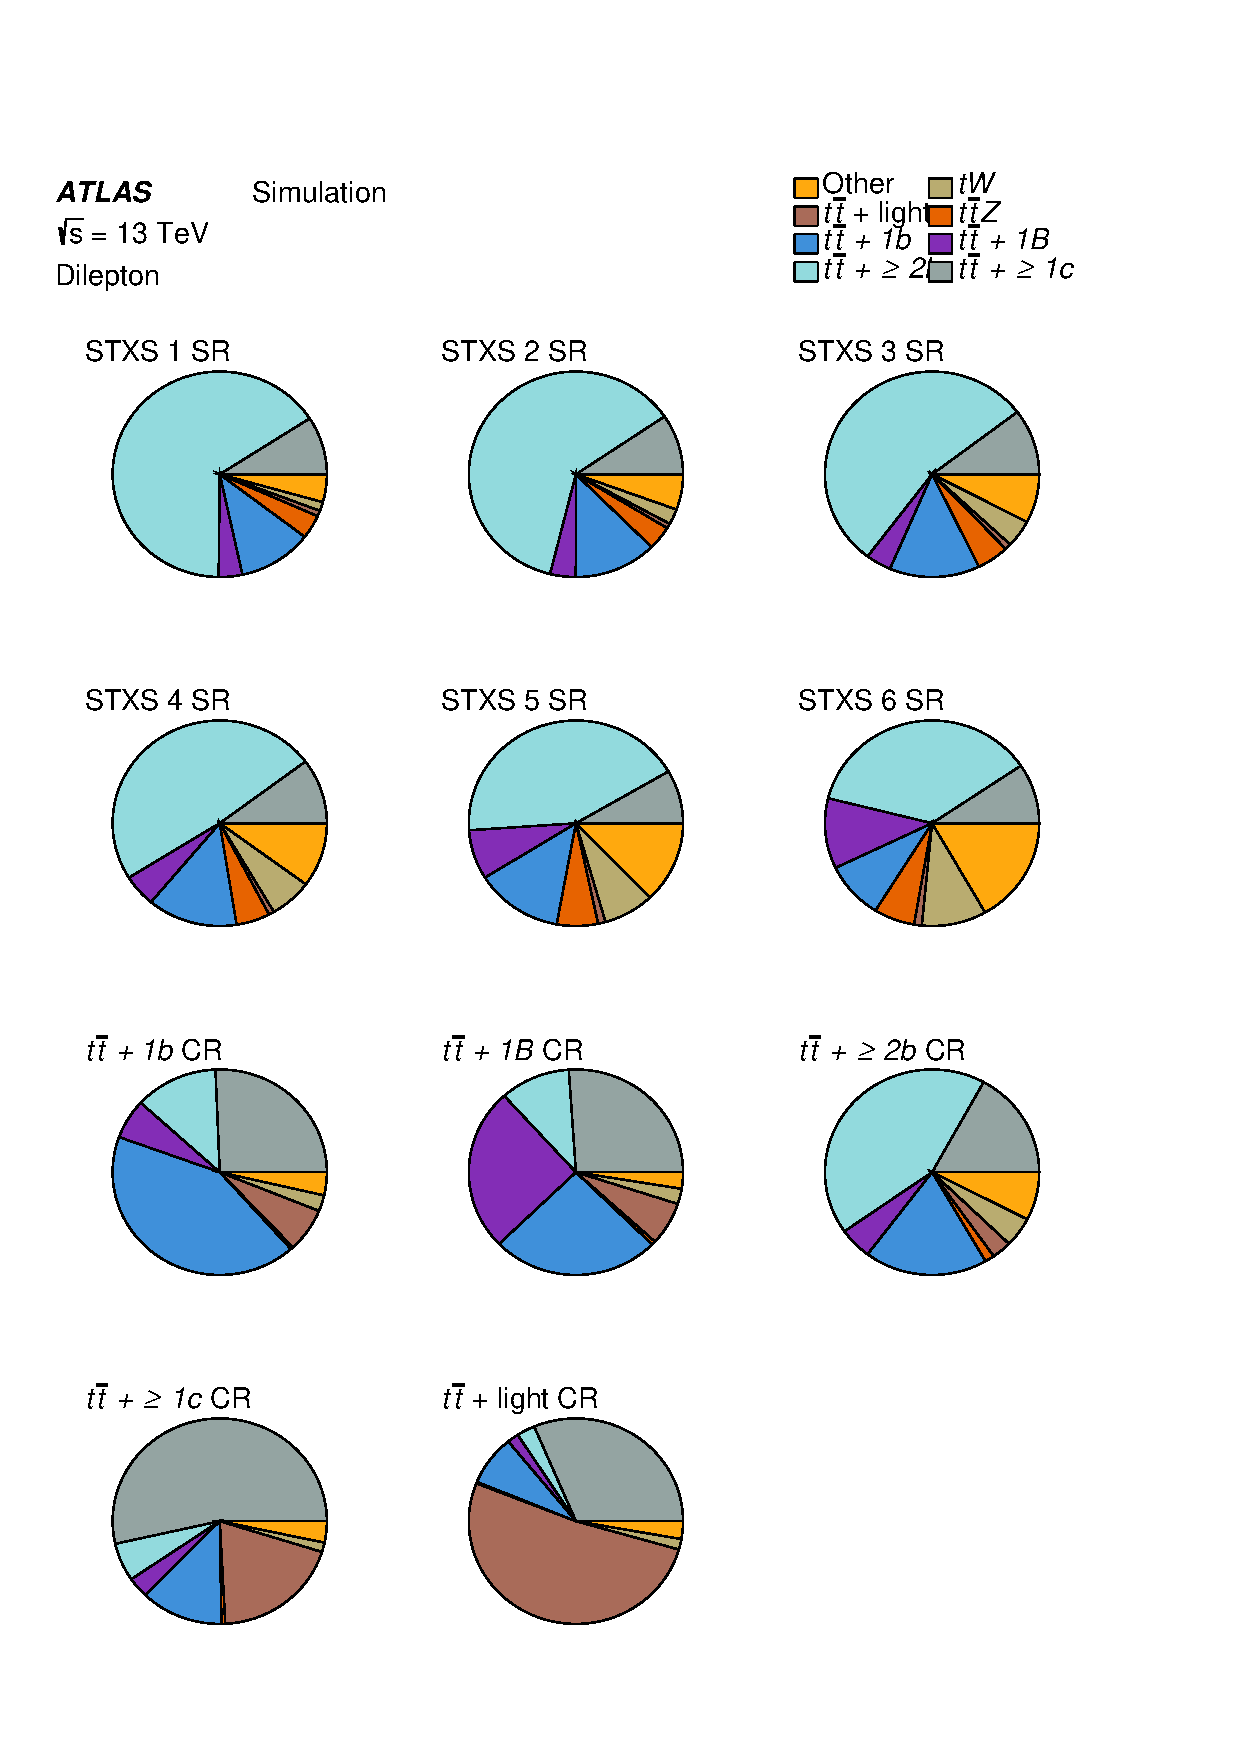
\includegraphics[width=0.9\linewidth]{Section_tthbb_analysis/figures/PrefitModel/dataMC_fit_regions/PieChart_2l.pdf}
    \caption{Composition of the background processes in the signal and control regions of the di-lepton channel. The pie charts display the relative contributions of all processes, with one chart per analysis region. Each control region is enriched in the corresponding output class of the transformer network, while the signal regions are further split according to $p_{T}^{H}$.  
}
    \label{fig:2l_region_comp}
\end{figure}
\begin{figure}[H]
    \centering
    % Row 1: 3 images
    \begin{subfigure}{0.3\textwidth}
        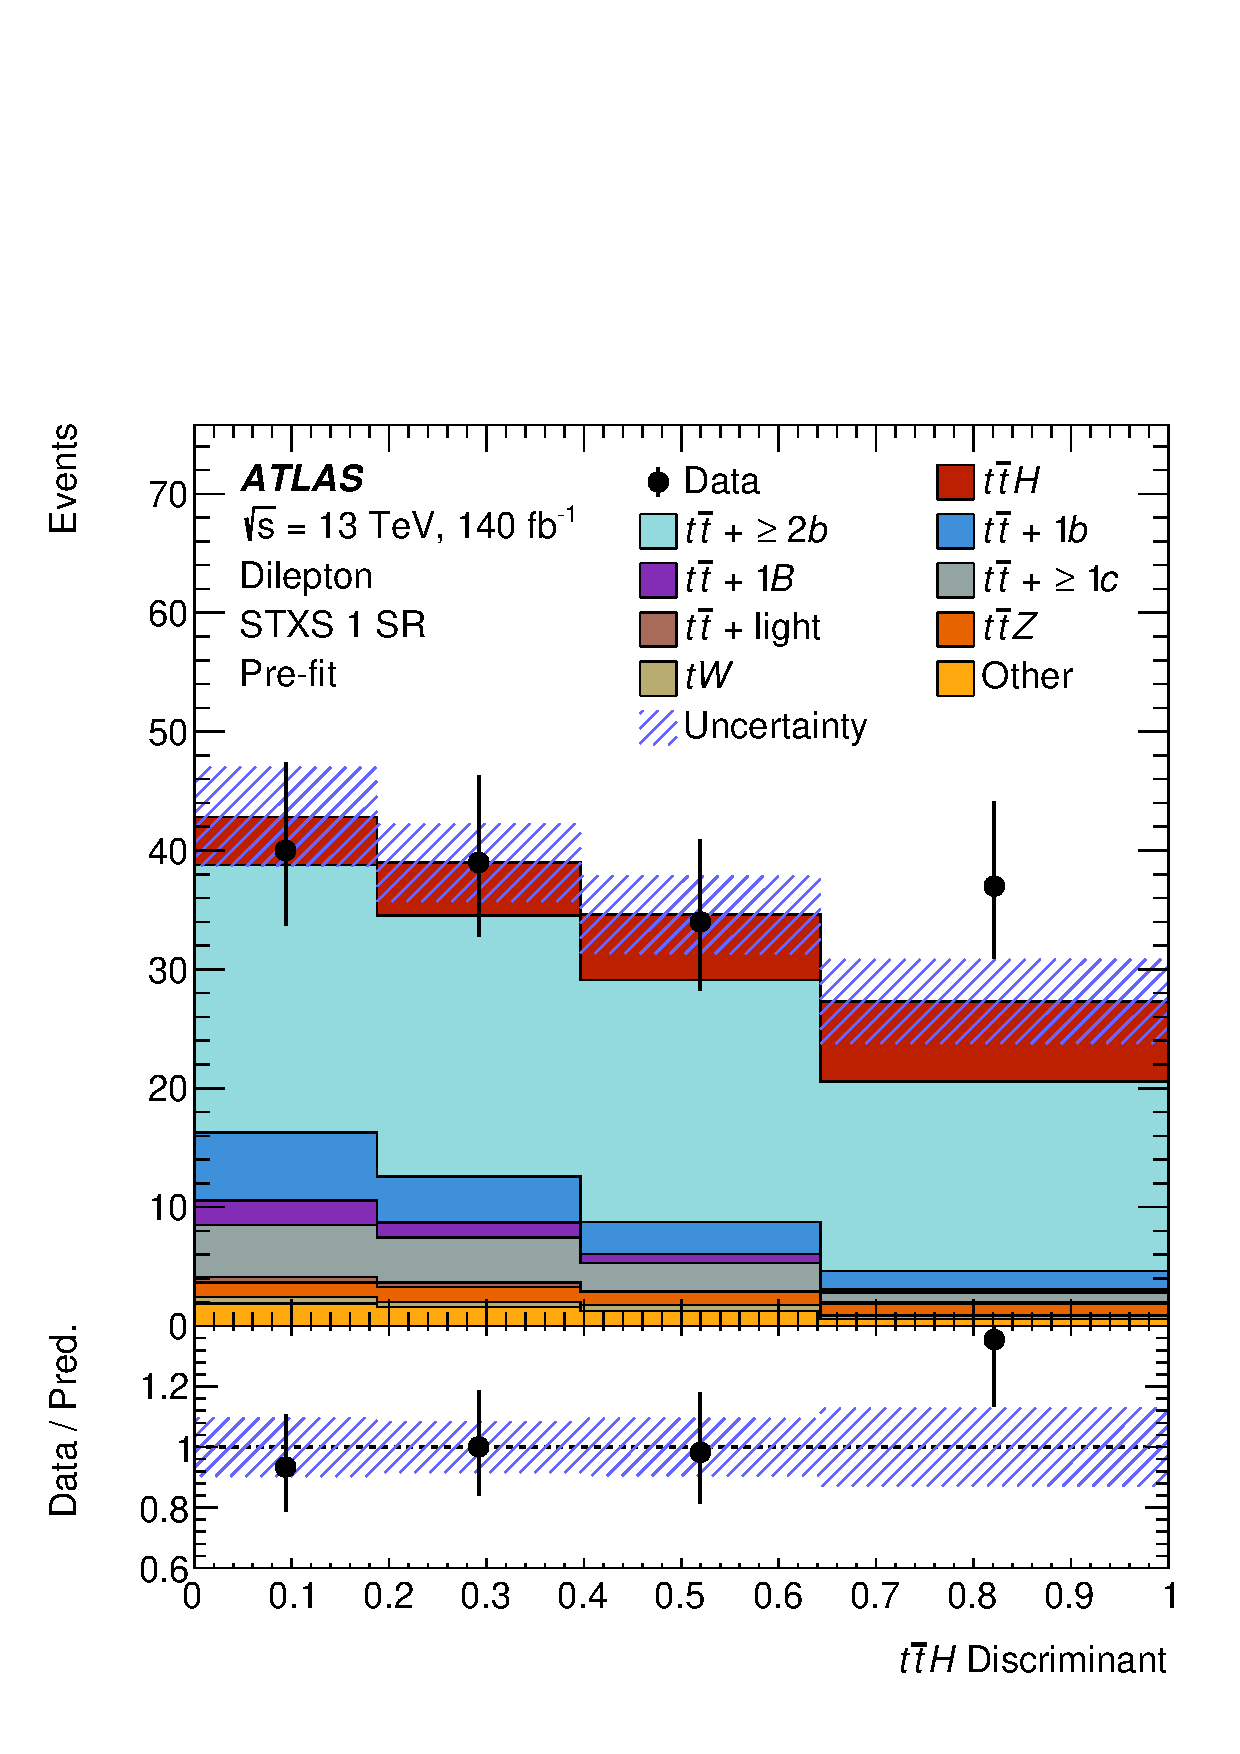
\includegraphics[width=\linewidth]{Section_tthbb_analysis/figures/Results/ttH_STXS1_2l.pdf}
        \caption{}
    \end{subfigure}
    \hfill
    \begin{subfigure}{0.3\textwidth}
        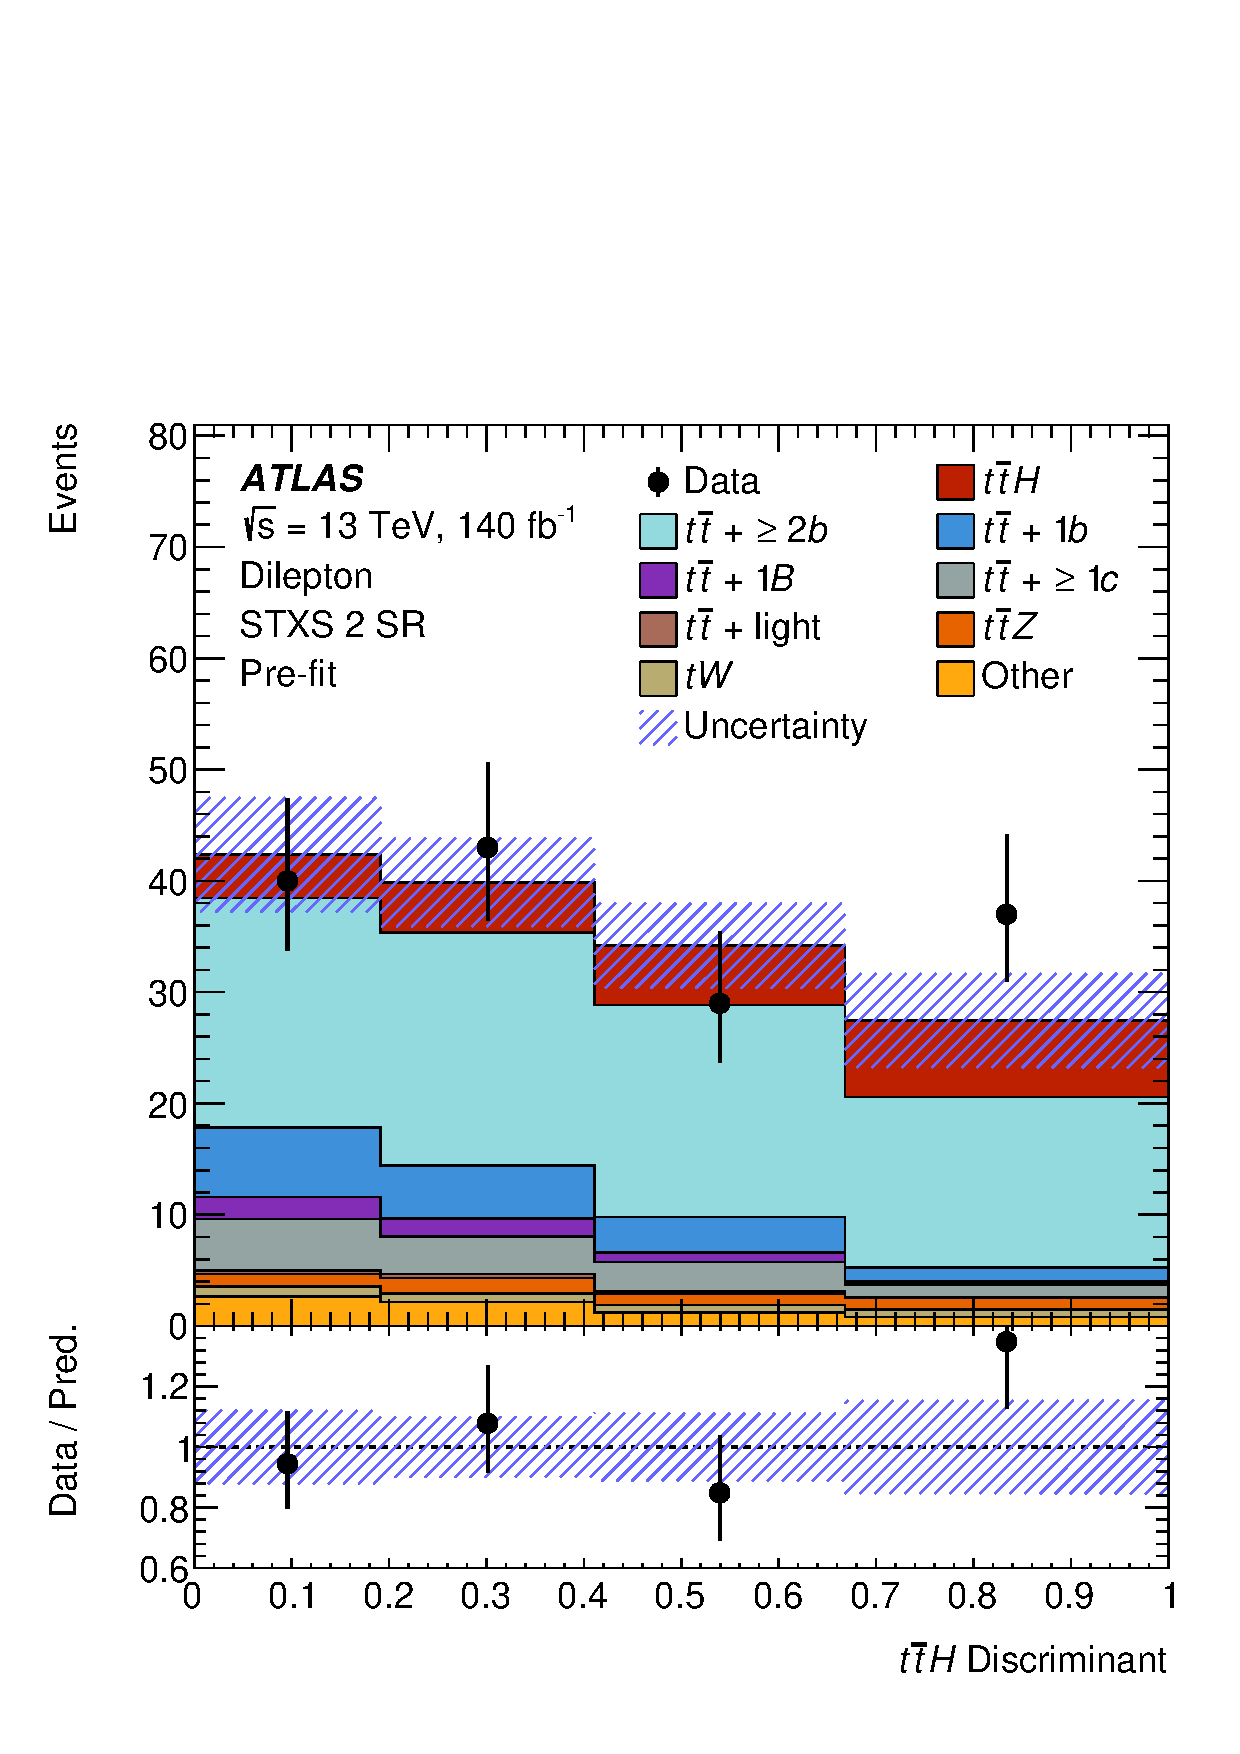
\includegraphics[width=\linewidth]{Section_tthbb_analysis/figures/Results/ttH_STXS2_2l.pdf}
        \caption{}
    \end{subfigure}
    \hfill
    \begin{subfigure}{0.3\textwidth}
        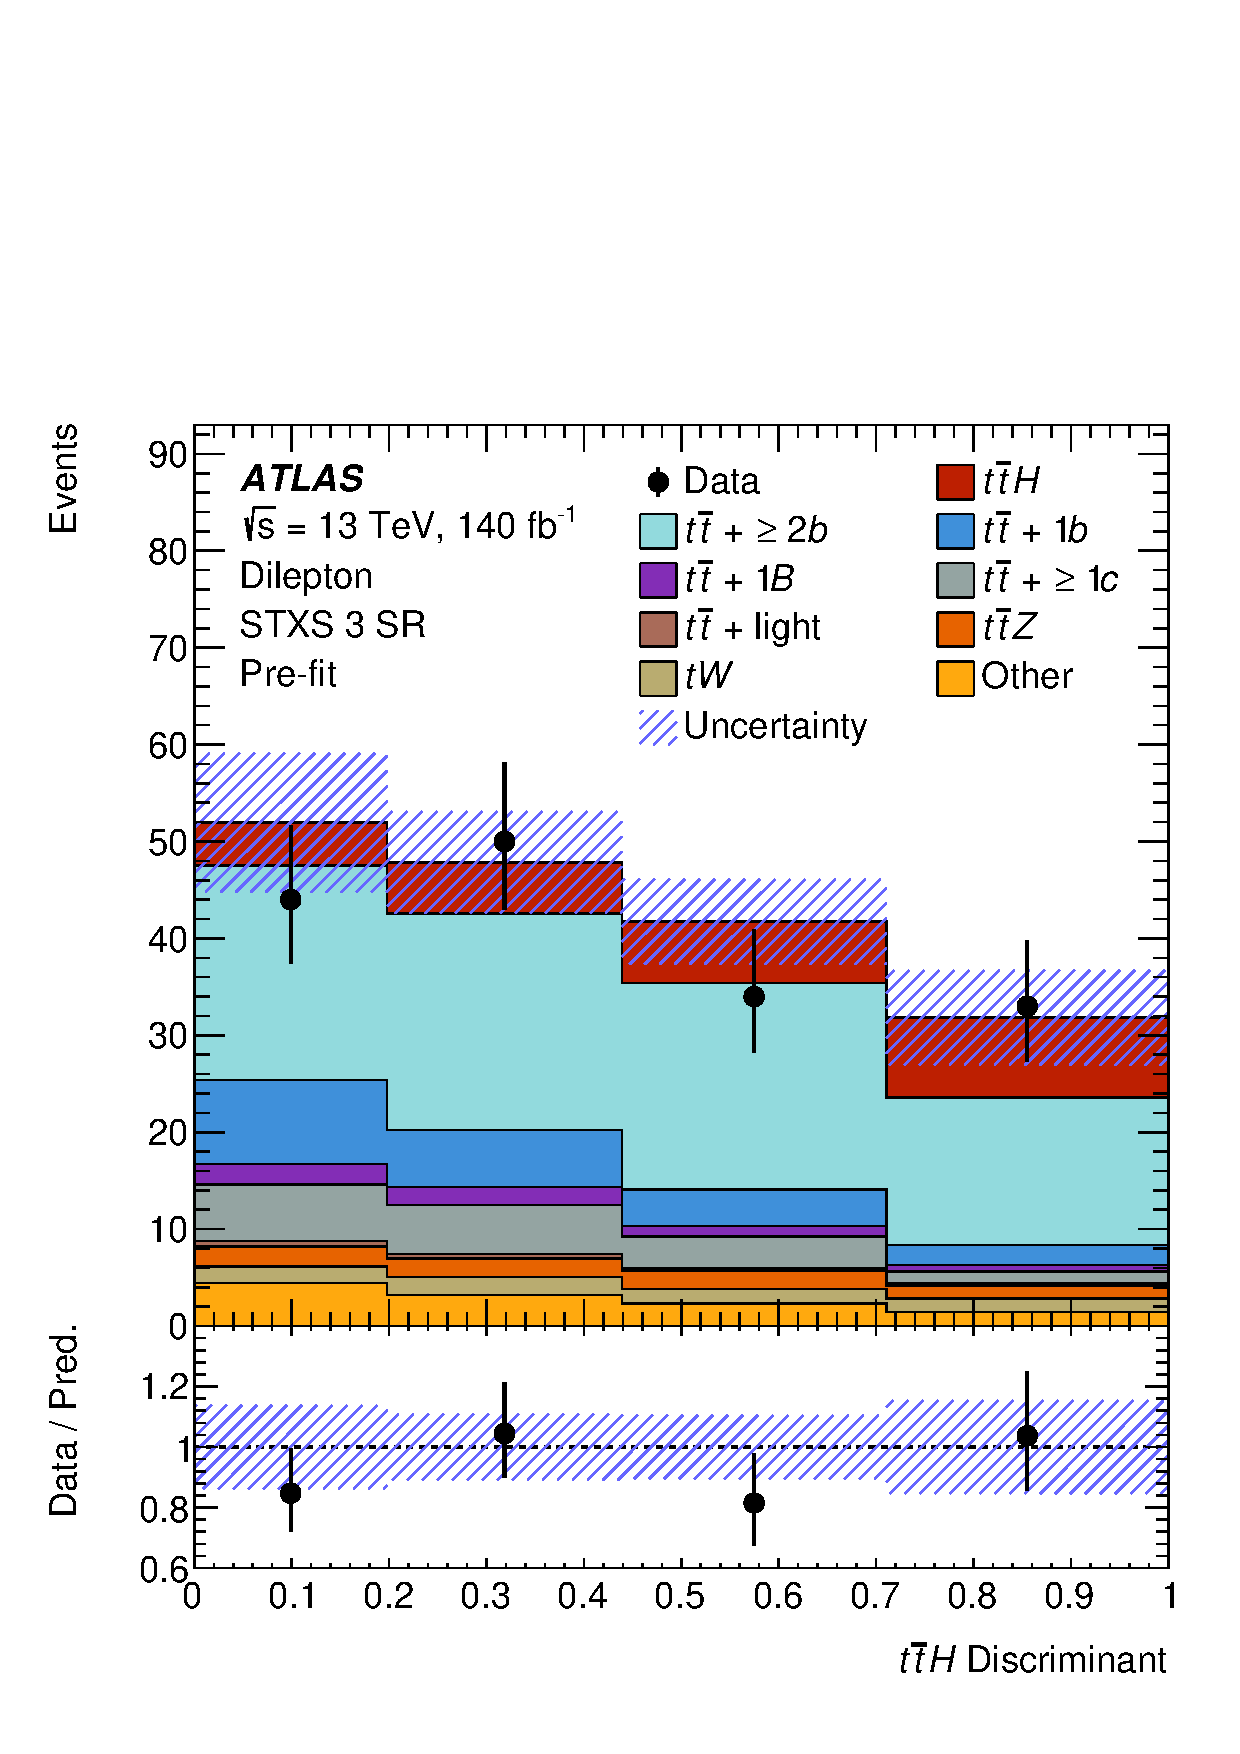
\includegraphics[width=\linewidth]{Section_tthbb_analysis/figures/Results/ttH_STXS3_2l.pdf}
        \caption{}
    \end{subfigure}
    
    \vspace{0.5cm} % space between rows
    
    % Row 2: 3 images
    \begin{subfigure}{0.3\textwidth}
        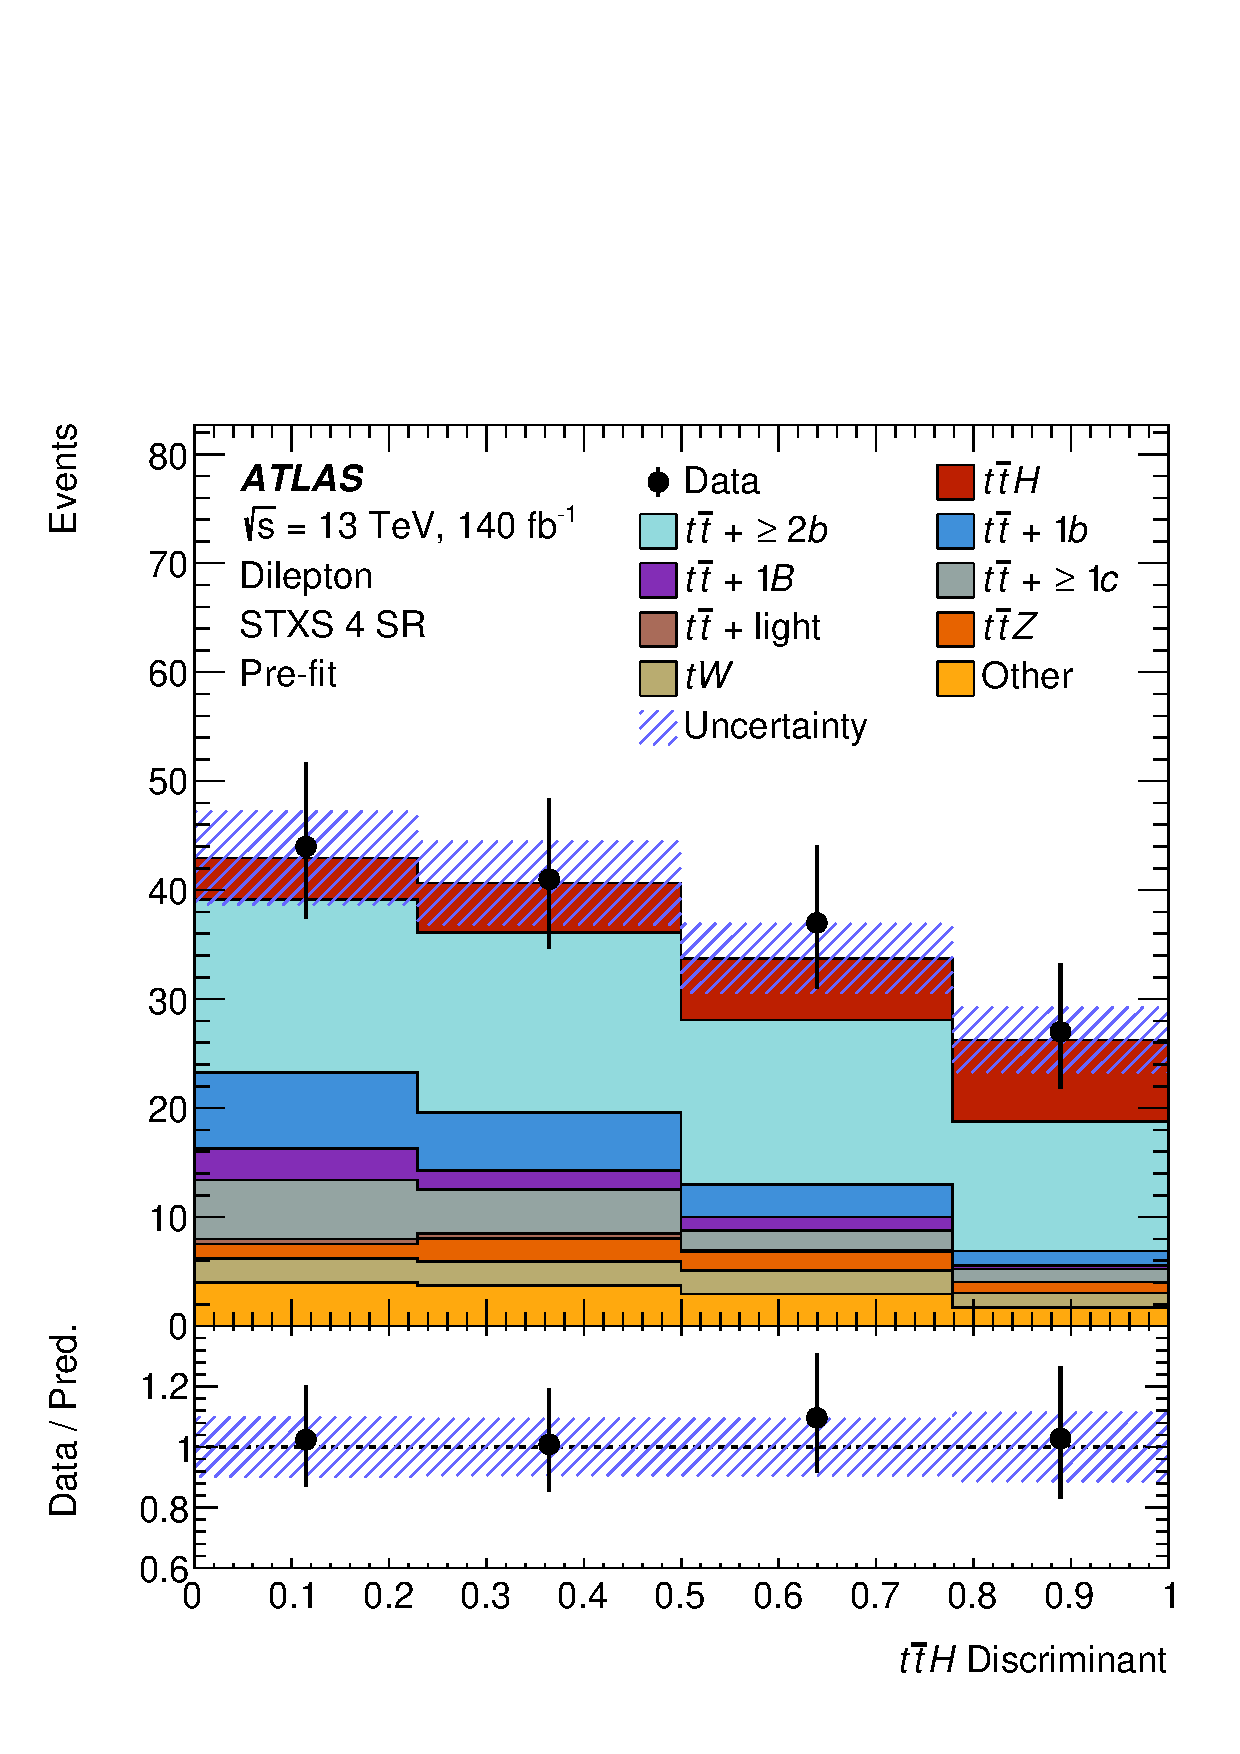
\includegraphics[width=\linewidth]{Section_tthbb_analysis/figures/Results/ttH_STXS4_2l.pdf}
        \caption{j}
    \end{subfigure}
    \hfill
    \begin{subfigure}{0.3\textwidth}
        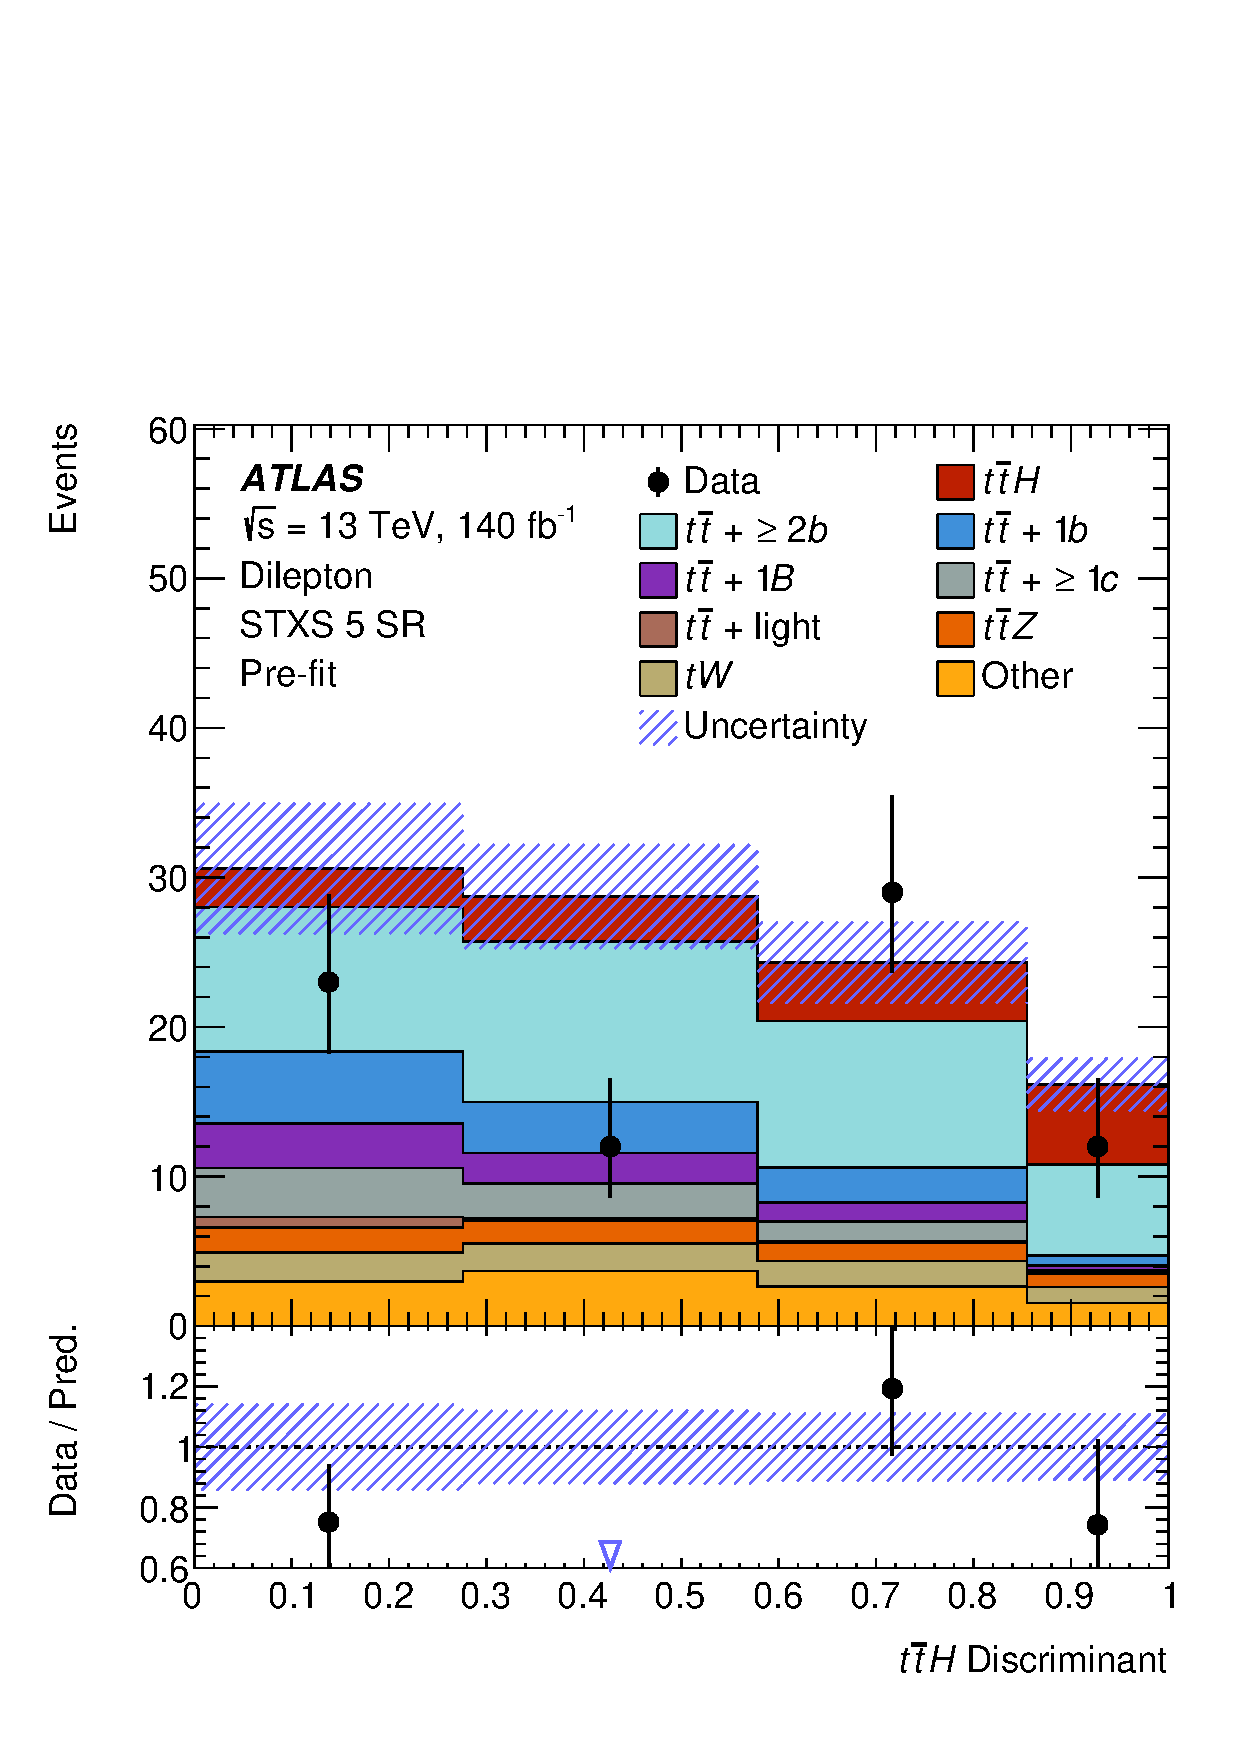
\includegraphics[width=\linewidth]{Section_tthbb_analysis/figures/Results/ttH_STXS5_2l.pdf}
        \caption{}
    \end{subfigure}
    \hfill
    \begin{subfigure}{0.3\textwidth}
        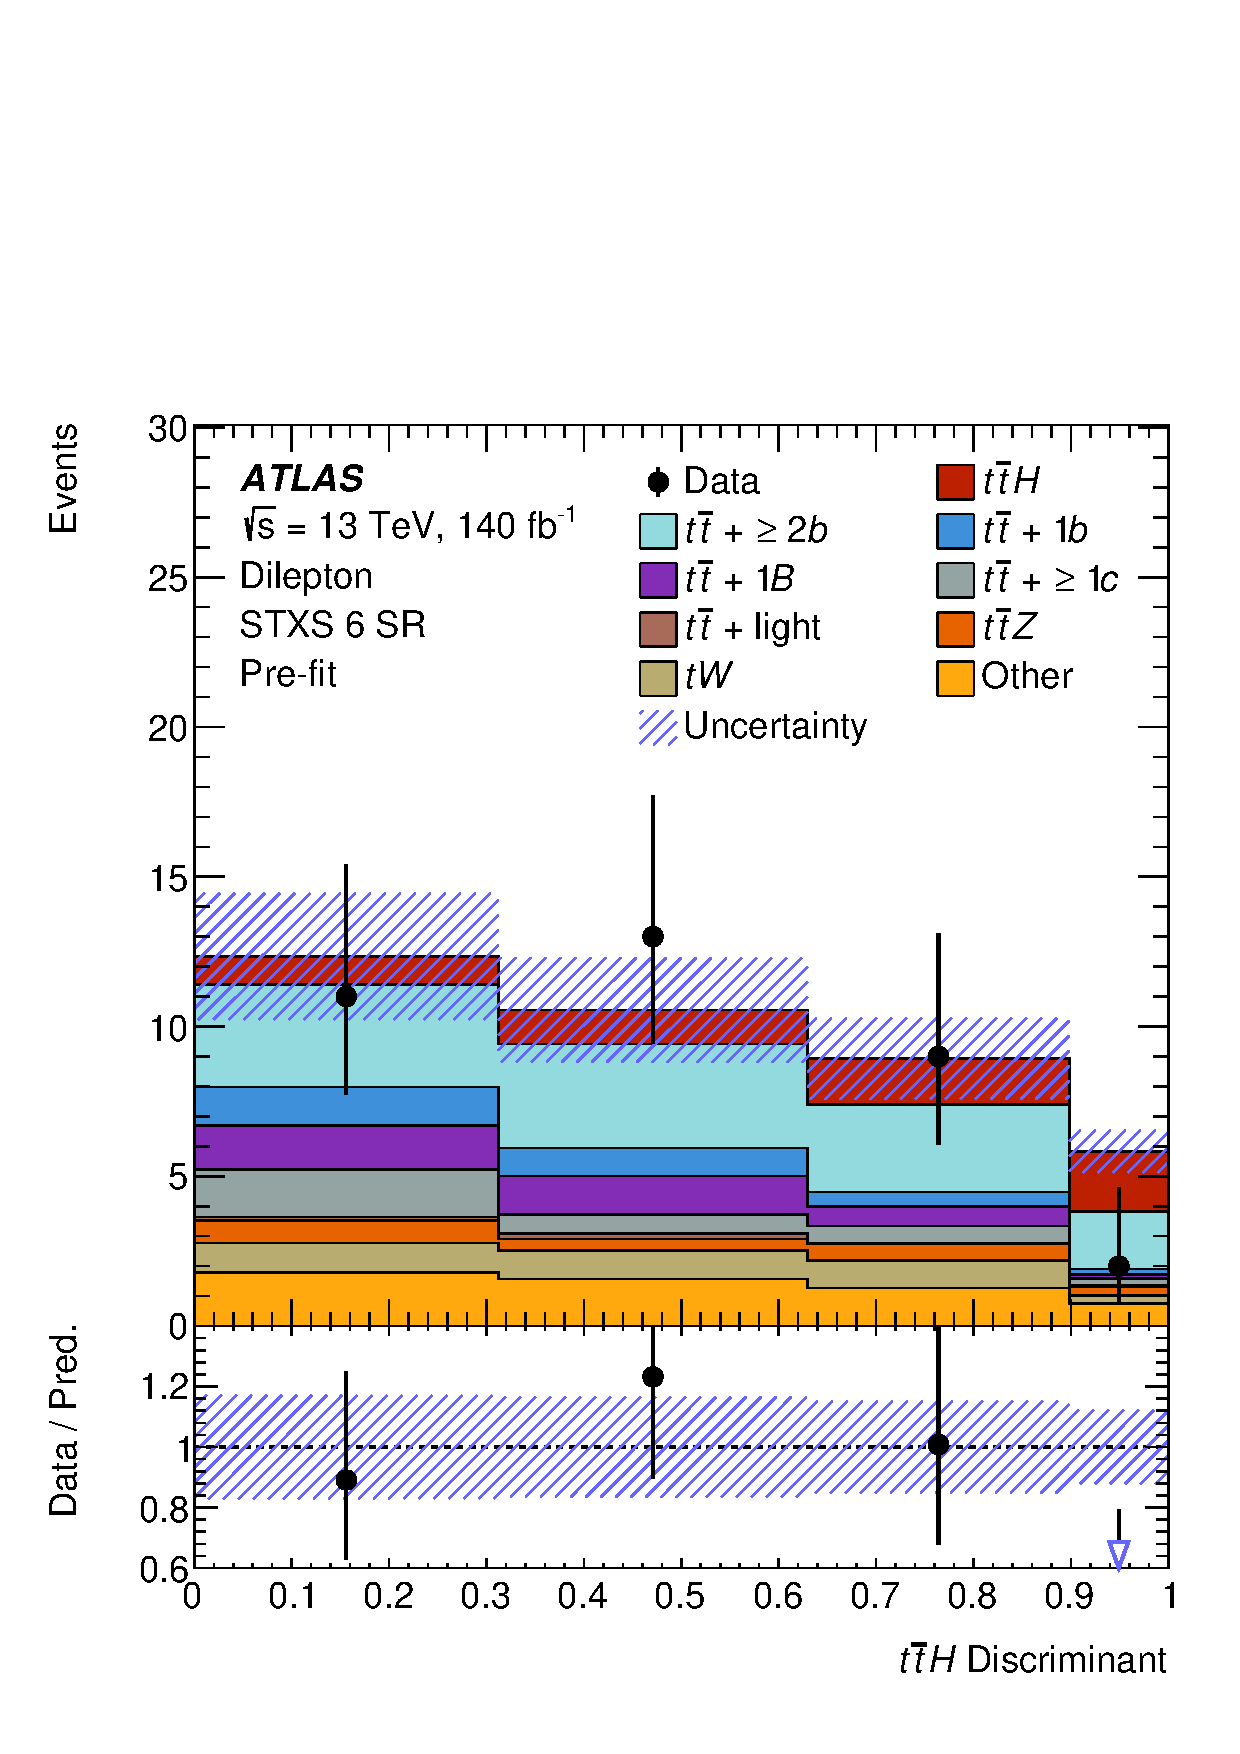
\includegraphics[width=\linewidth]{Section_tthbb_analysis/figures/Results/ttH_STXS6_2l.pdf}
        \caption{}
    \end{subfigure}
    
    \vspace{0.5cm} % space before last row
    
    % Row 3: 1 centered image

    
    \caption{Pre-fit distributions of the six signal regions in the dilepton channel: (a) STXS 1, (b) STXS 2, (c) STXS 3, (d) STXS 4, (e) STXS 5, (f) STXS 6. Each region is constructed to be enriched in the relevant flavour component of the additional jets in the dominant $t\bar{t}+$jets background. The uncertainty band includes both statistical and systematic contributions, excluding the free-floating normalisations of the individual $t\bar{t}+$jets flavour components. All discriminant scores are rescaled to the interval $[0,1]$ using a logistic function.}
    \label{fig:2l_data_mc_pre_fit_SR}
\end{figure}
\begin{figure}[H]
    \centering
    % Row 1: 3 images
    \begin{subfigure}{0.3\textwidth}
        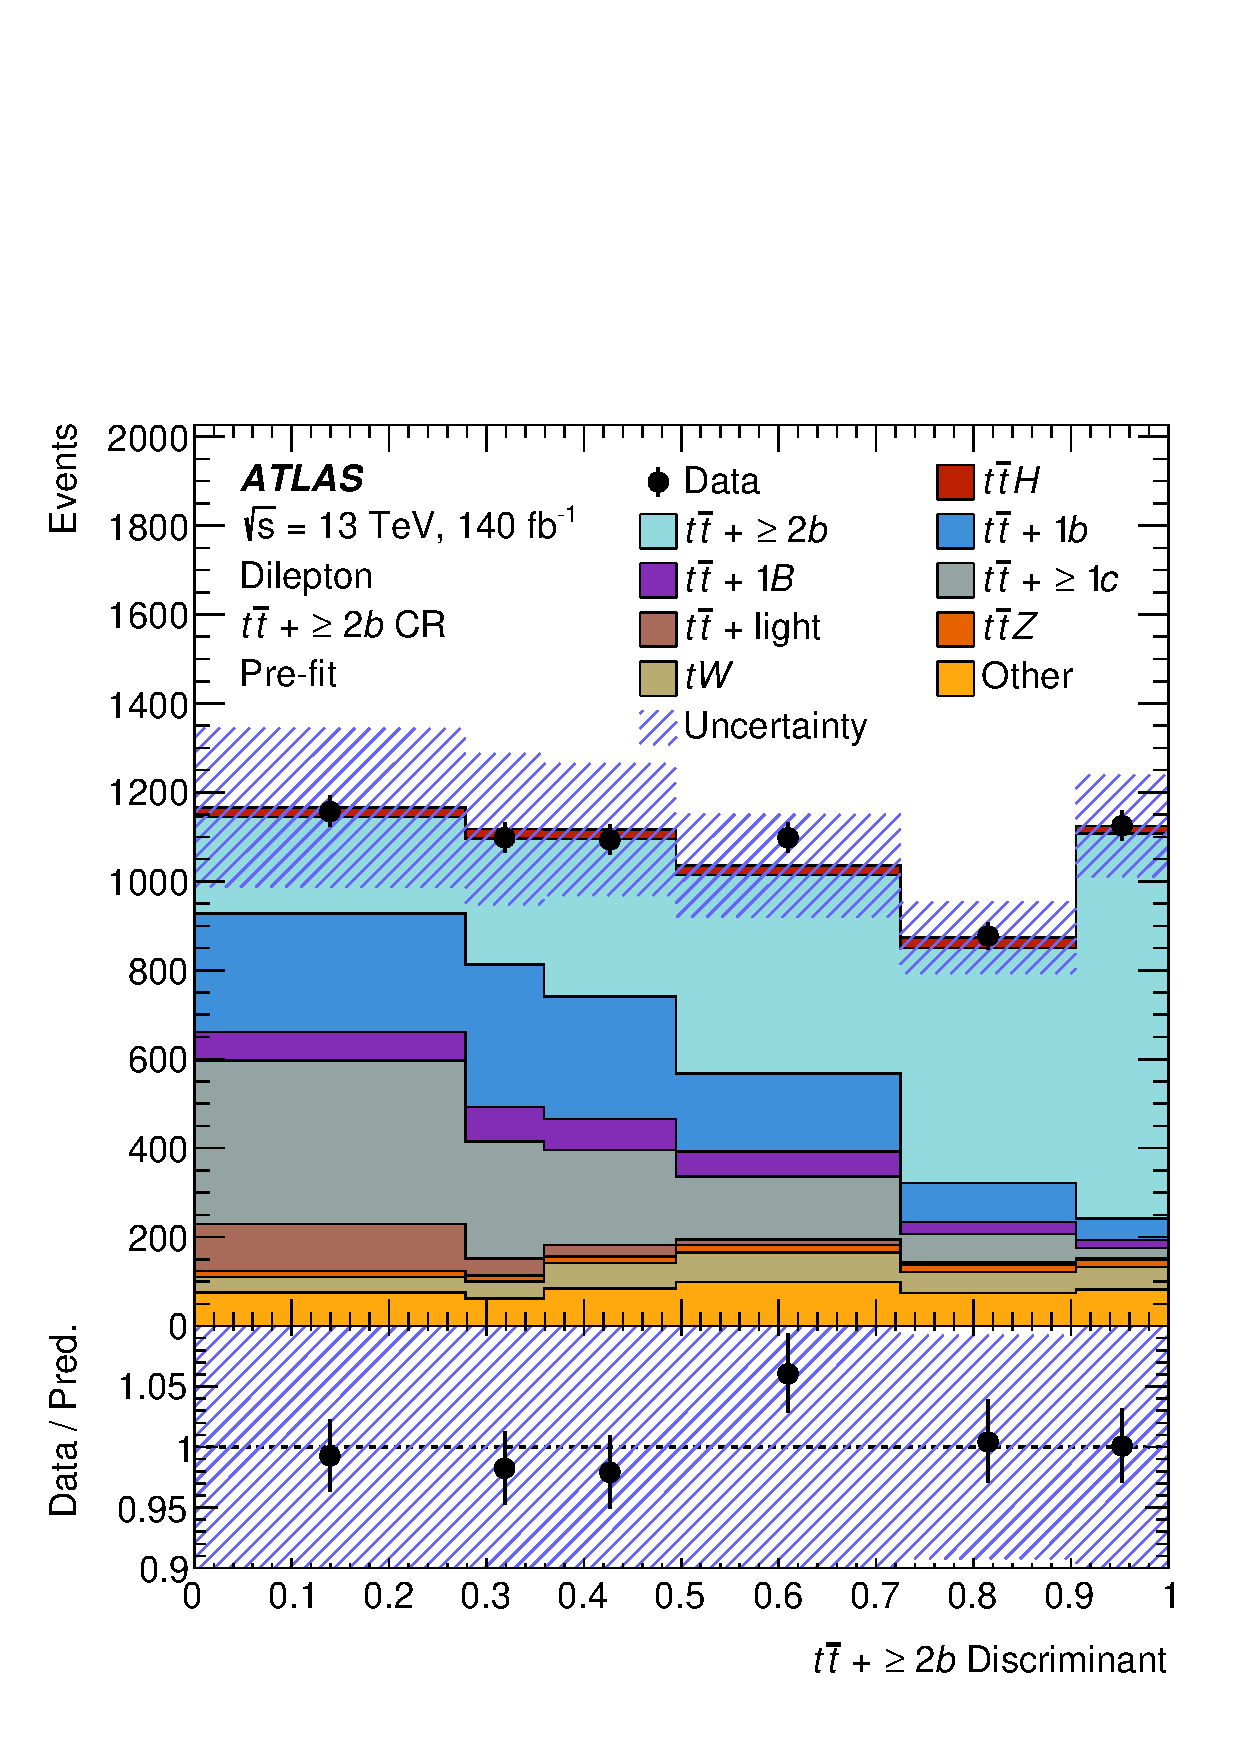
\includegraphics[width=\linewidth]{Section_tthbb_analysis/figures/Results/tt2b_2l.pdf}
        \caption{}
    \end{subfigure}
\hfill
    \begin{subfigure}{0.3\textwidth}
        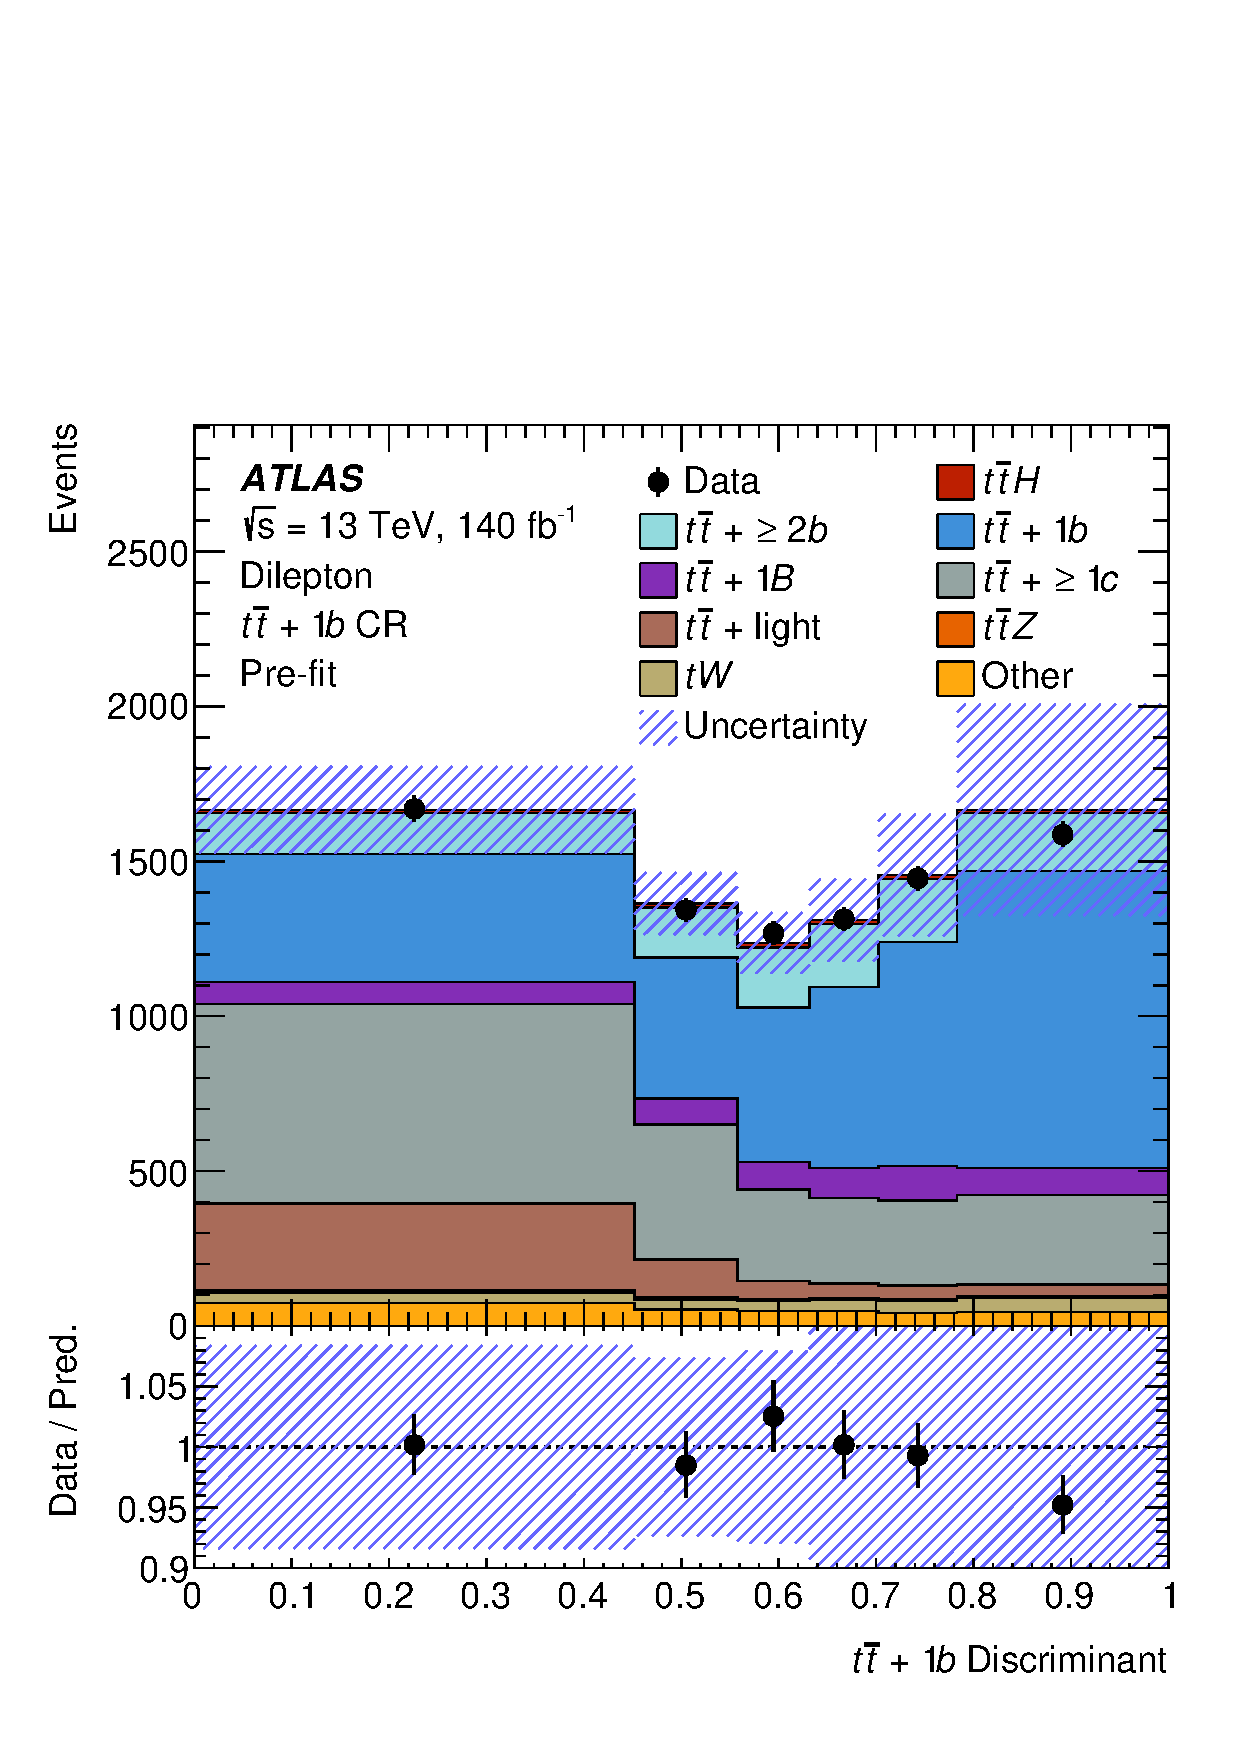
\includegraphics[width=\linewidth]{Section_tthbb_analysis/figures/Results/tt1b_2l.pdf}
        \caption{j}
    \end{subfigure}
    \hfill
    \begin{subfigure}{0.3\textwidth}
        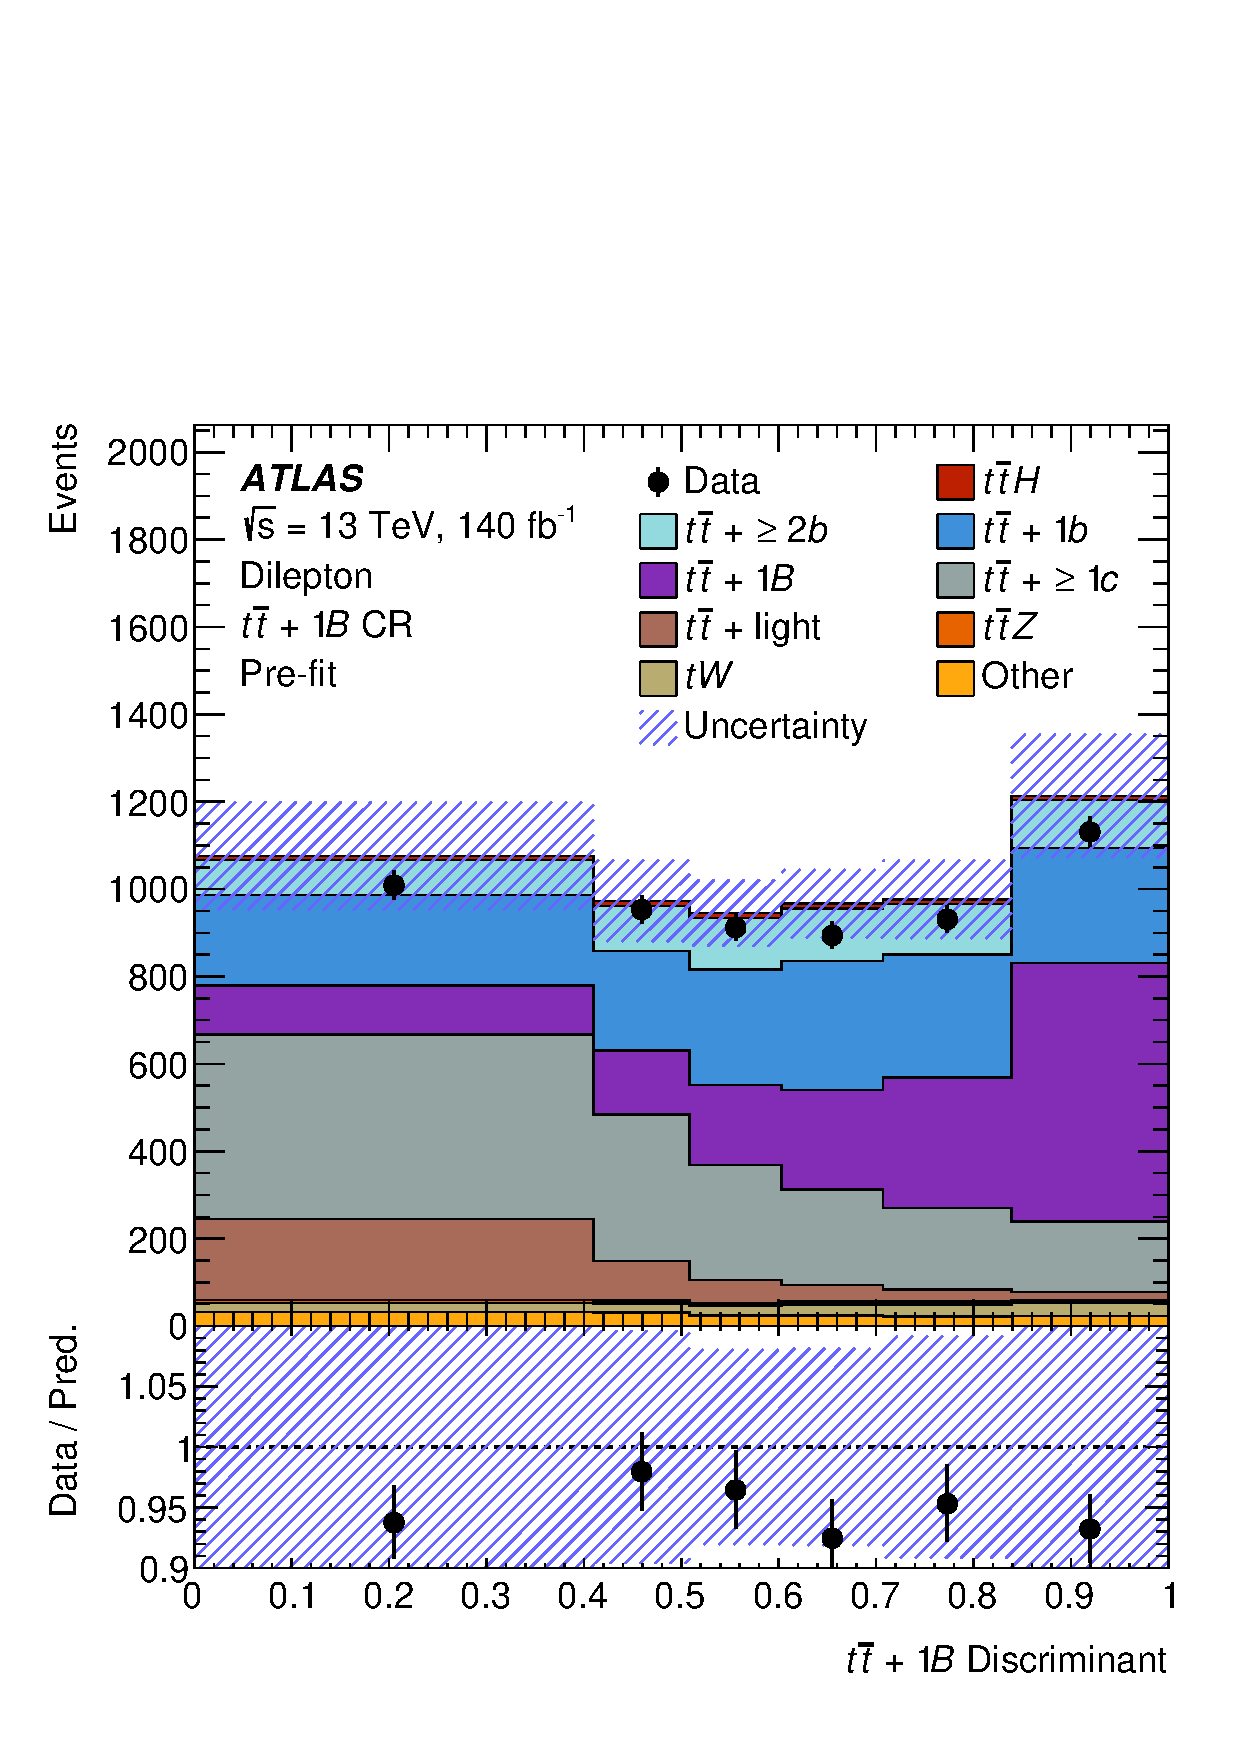
\includegraphics[width=\linewidth]{Section_tthbb_analysis/figures/Results/ttB_2l.pdf}
        \caption{}
    \end{subfigure}
    \vspace{0.5cm}
    \begin{subfigure}{0.3\textwidth}
        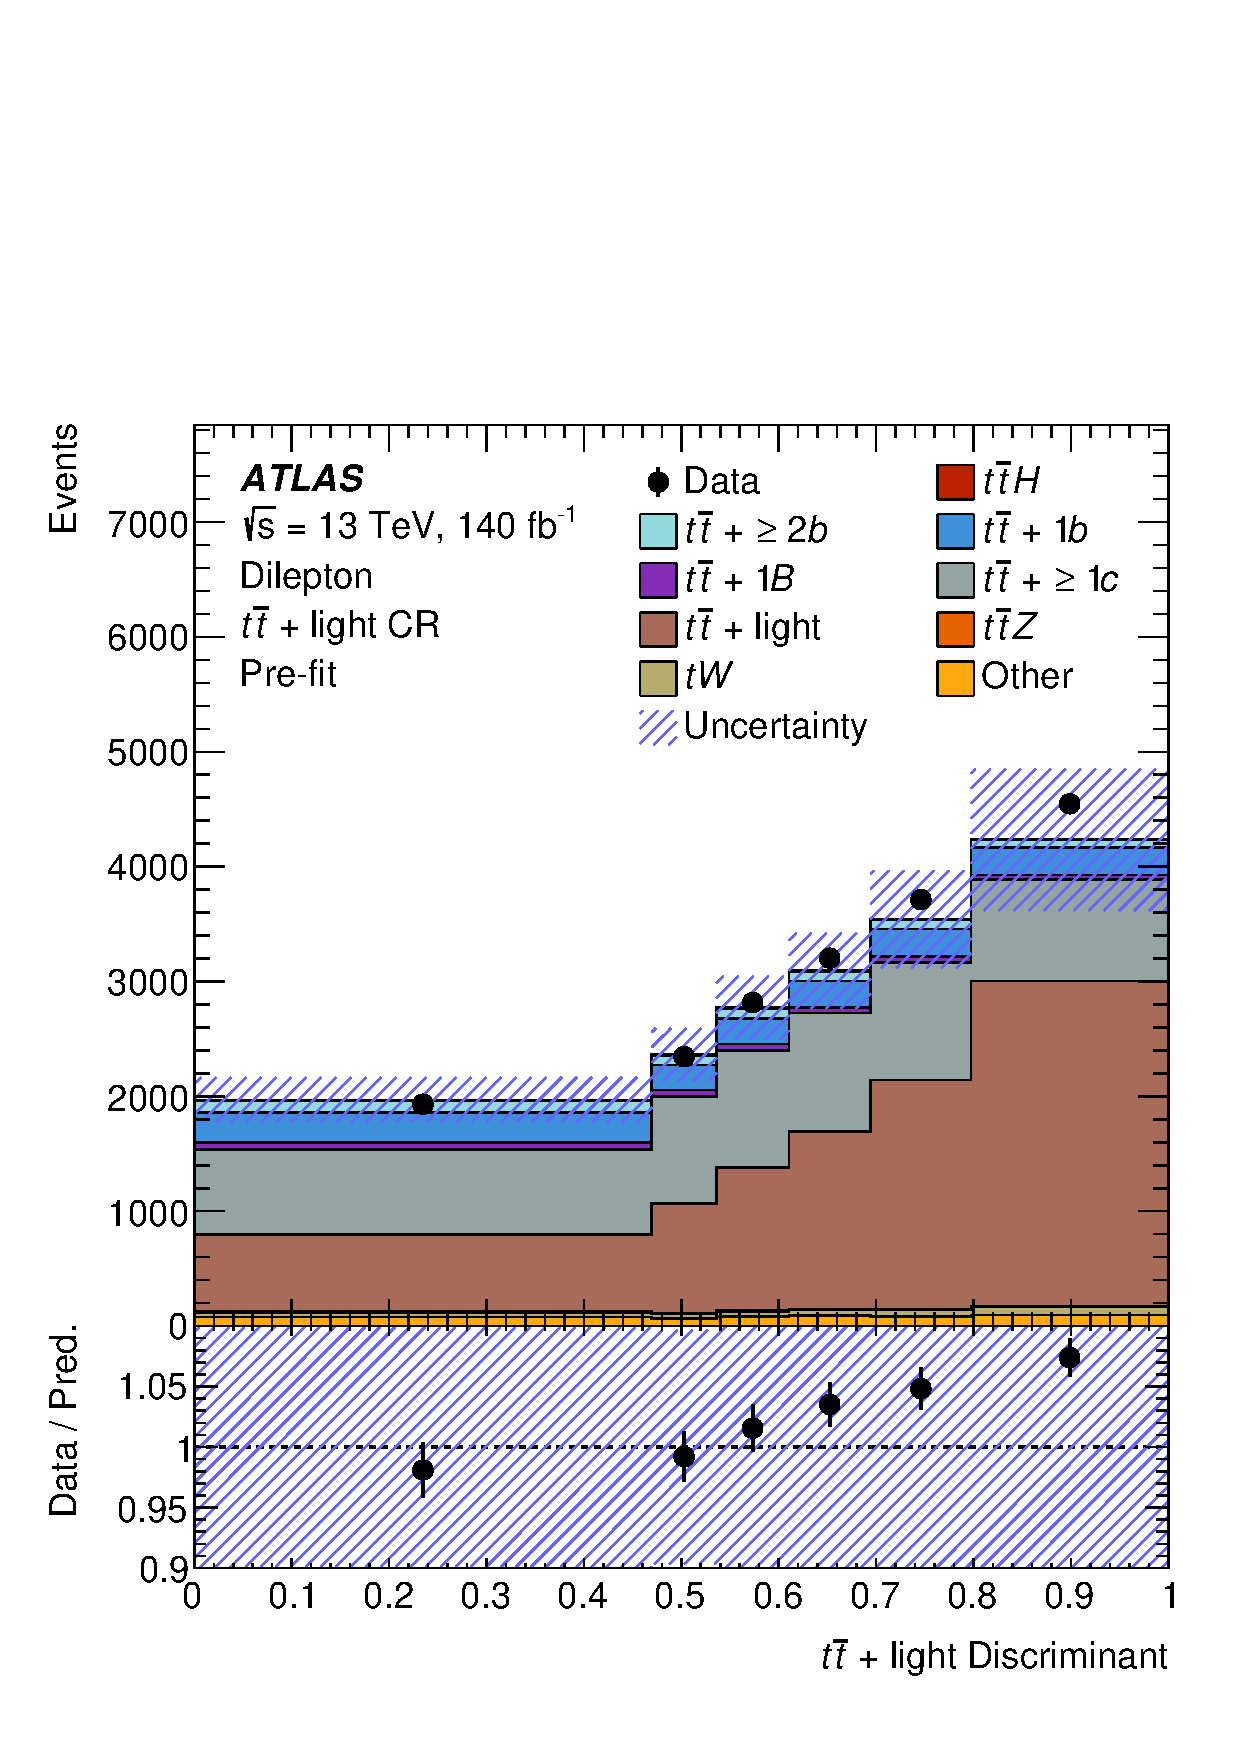
\includegraphics[width=\linewidth]{Section_tthbb_analysis/figures/Results/tt_light_2l.pdf}
        \caption{}
    \end{subfigure}
\hspace{0.1\textwidth}
    \begin{subfigure}{0.3\textwidth}
        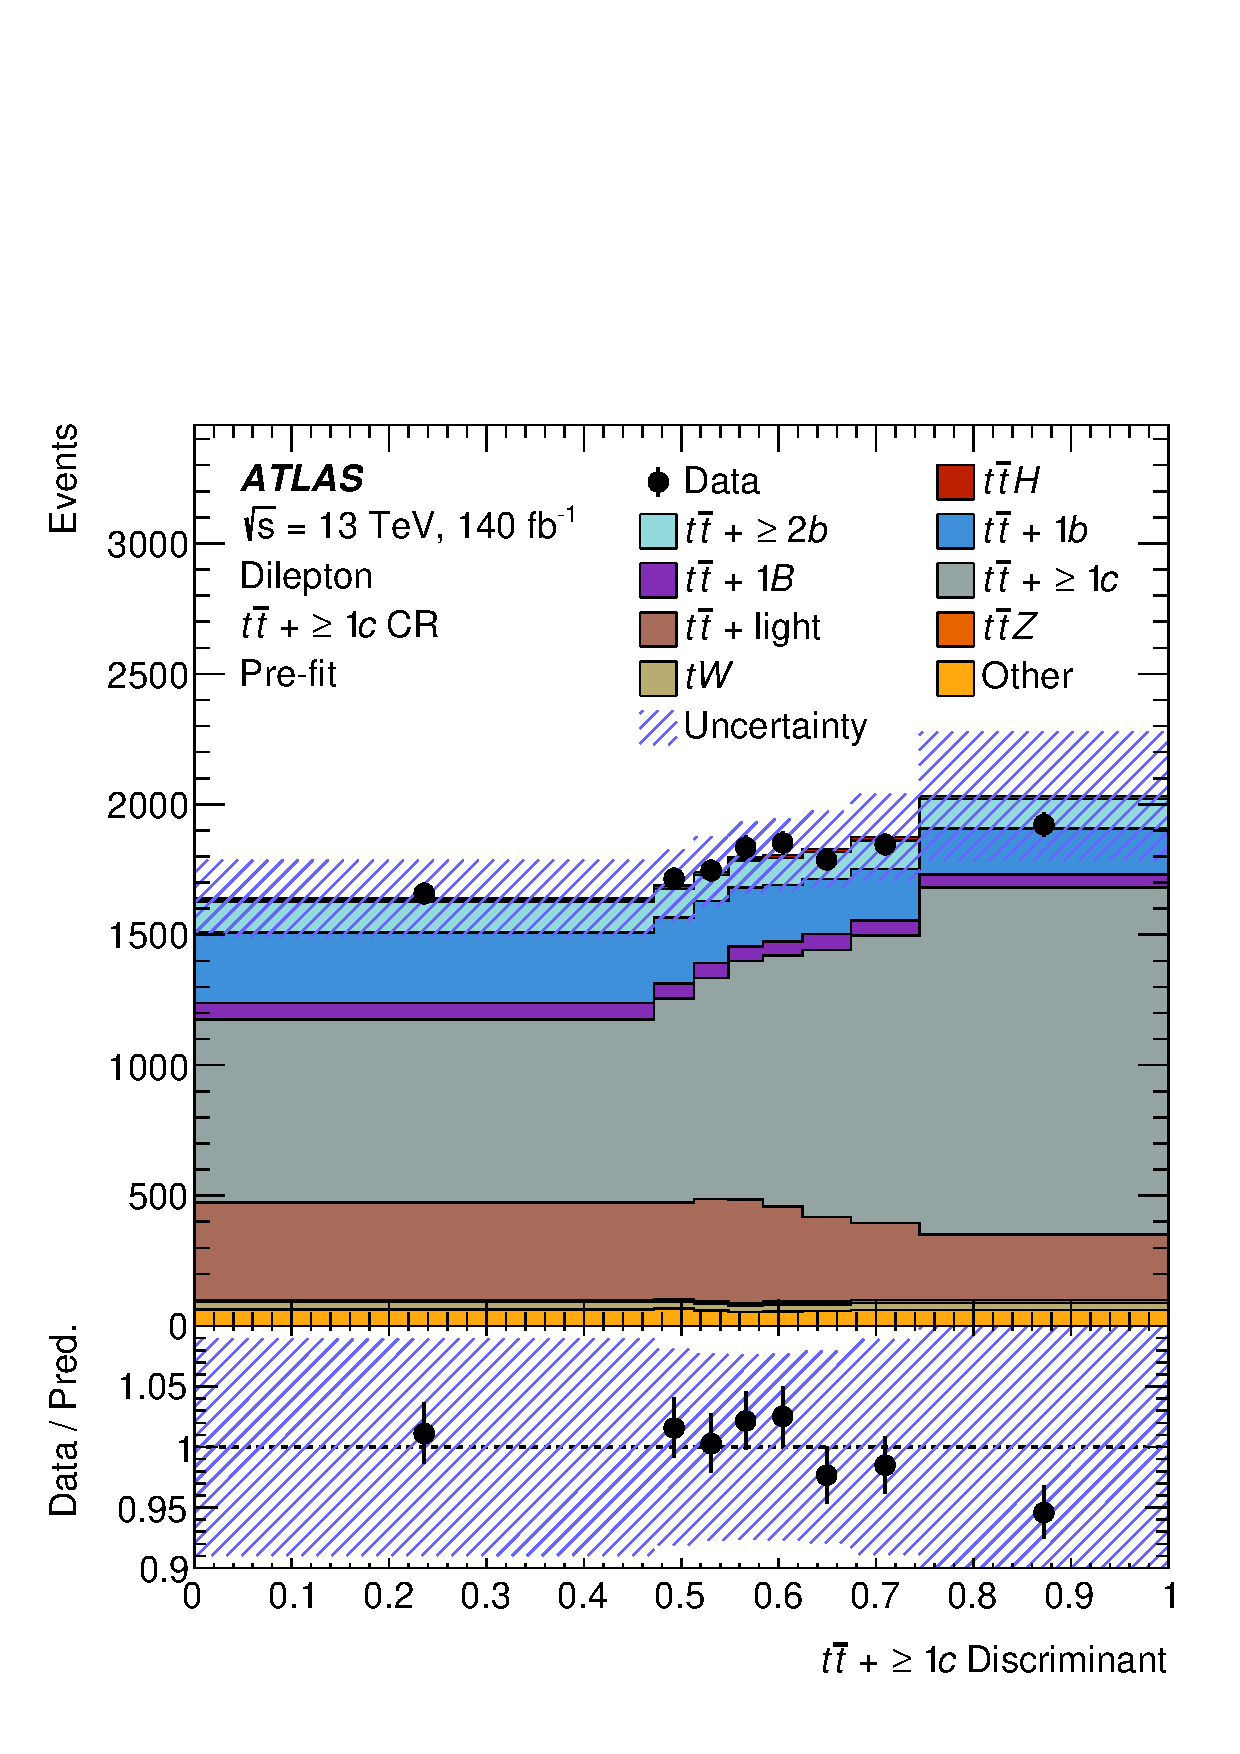
\includegraphics[width=\linewidth]{Section_tthbb_analysis/figures/Results/ttc_2l.pdf}
        \caption{}
    \end{subfigure}

    
    \caption{Pre-fit distributions of the six control regions in the di-lepton channel: (a) $t\bar{t}+\geq 2b$, (b) $t\bar{t}+1b$, (c) $t\bar{t}+1B$, (d) $t\bar{t}+$light, (e) $t\bar{t}+\geq 1c$. Each region is constructed to be enriched in the corresponding flavour component of the additional jets in the dominant $t\bar{t}+$jets background. The uncertainty band includes both statistical and systematic contributions, excluding the free-floating normalisations of the individual $t\bar{t}+$jets flavour components. All discriminant scores are rescaled to the interval $[0,1]$ using a logistic function.}
    \label{fig:2l_data_mc_pre_fit_CR}
\end{figure}
\section{Post-Fit Modelling}
\begin{figure}[!htb]
    \centering
    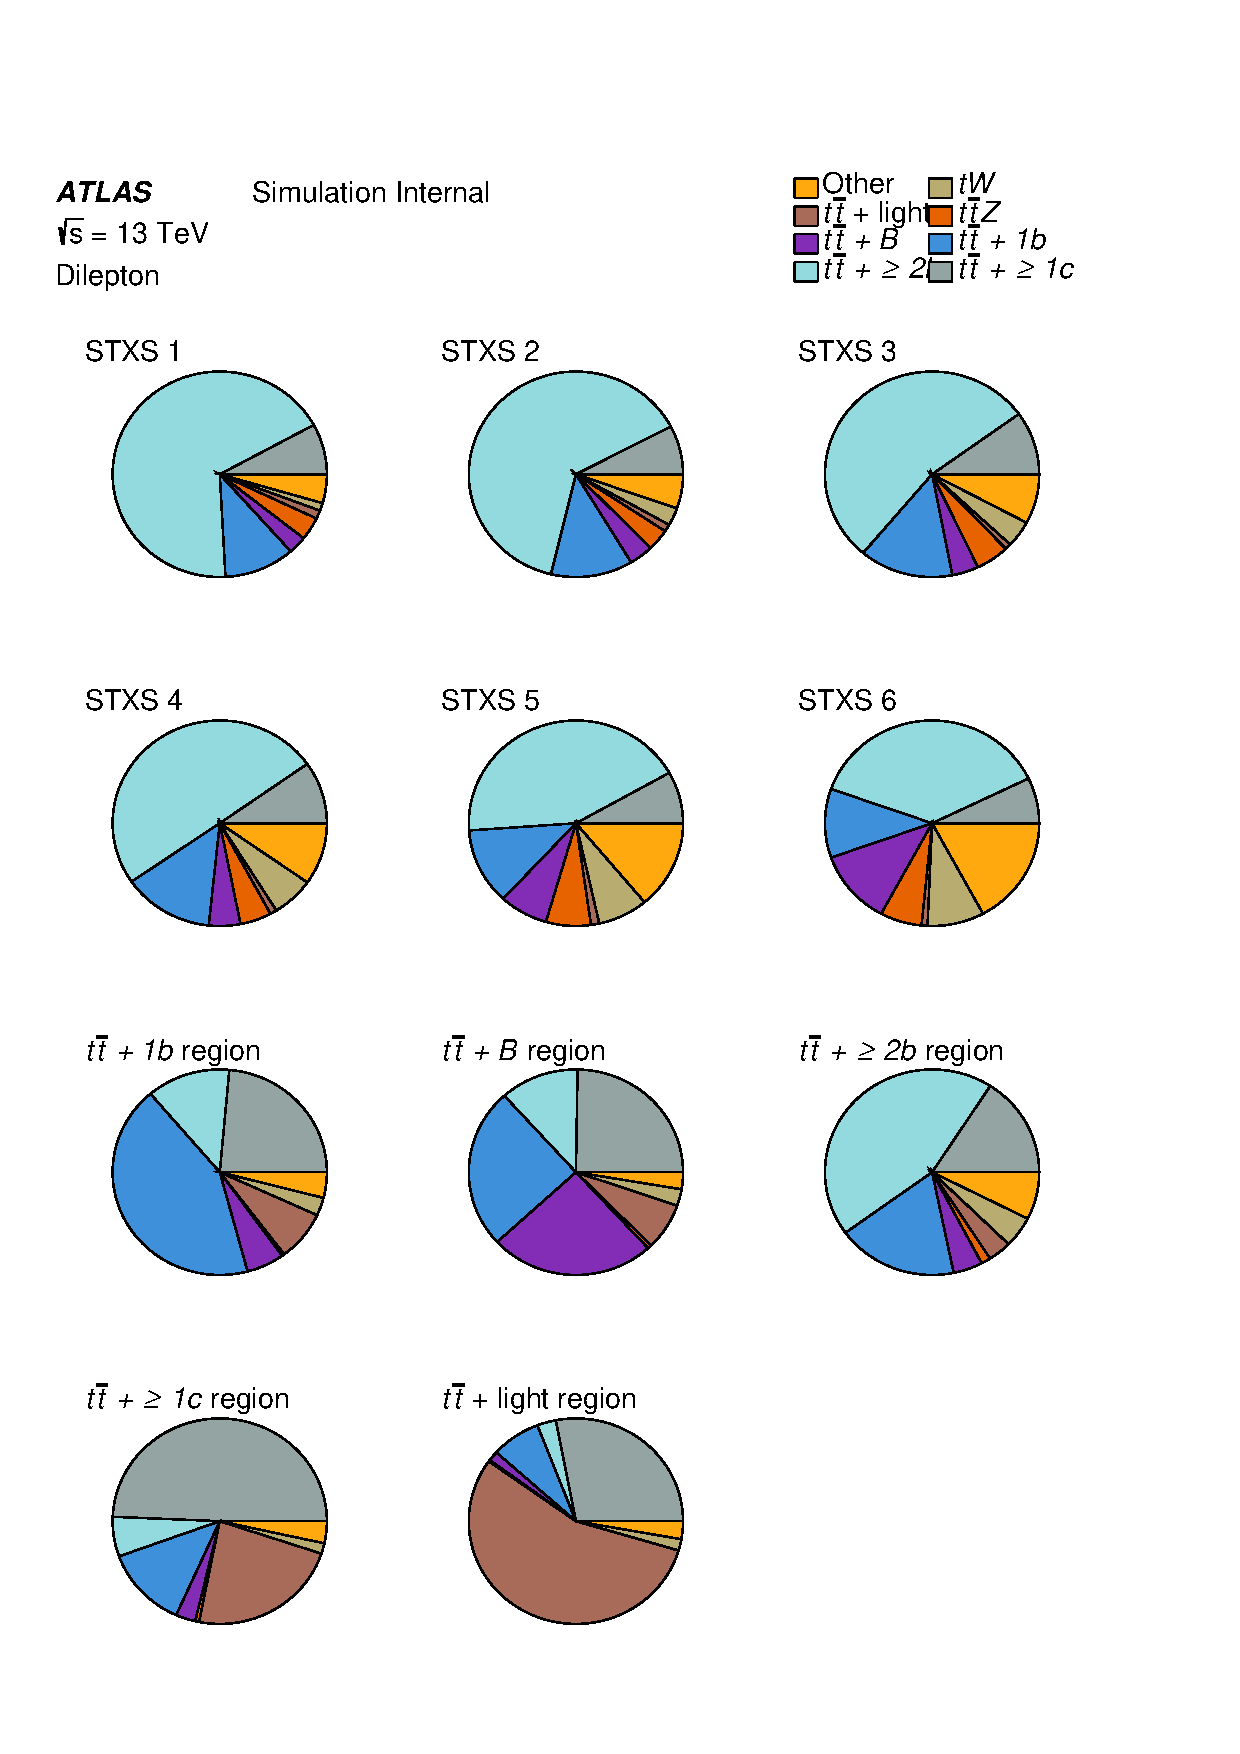
\includegraphics[width=0.6\linewidth]{Section_tthbb_analysis/figures/Results/PieChart_dil_postFit.pdf}
    \caption{Composition of the signal and control regions of the di-lepton channel. The pie charts indicate the relative contributions of all processes, with one chart per analysis region.  
}
    \label{fig:2l_region_comp_post_fit}
\end{figure}
\begin{figure}[!htb]
    \centering
    % Row 1: 3 images
    \begin{subfigure}{0.3\textwidth}
        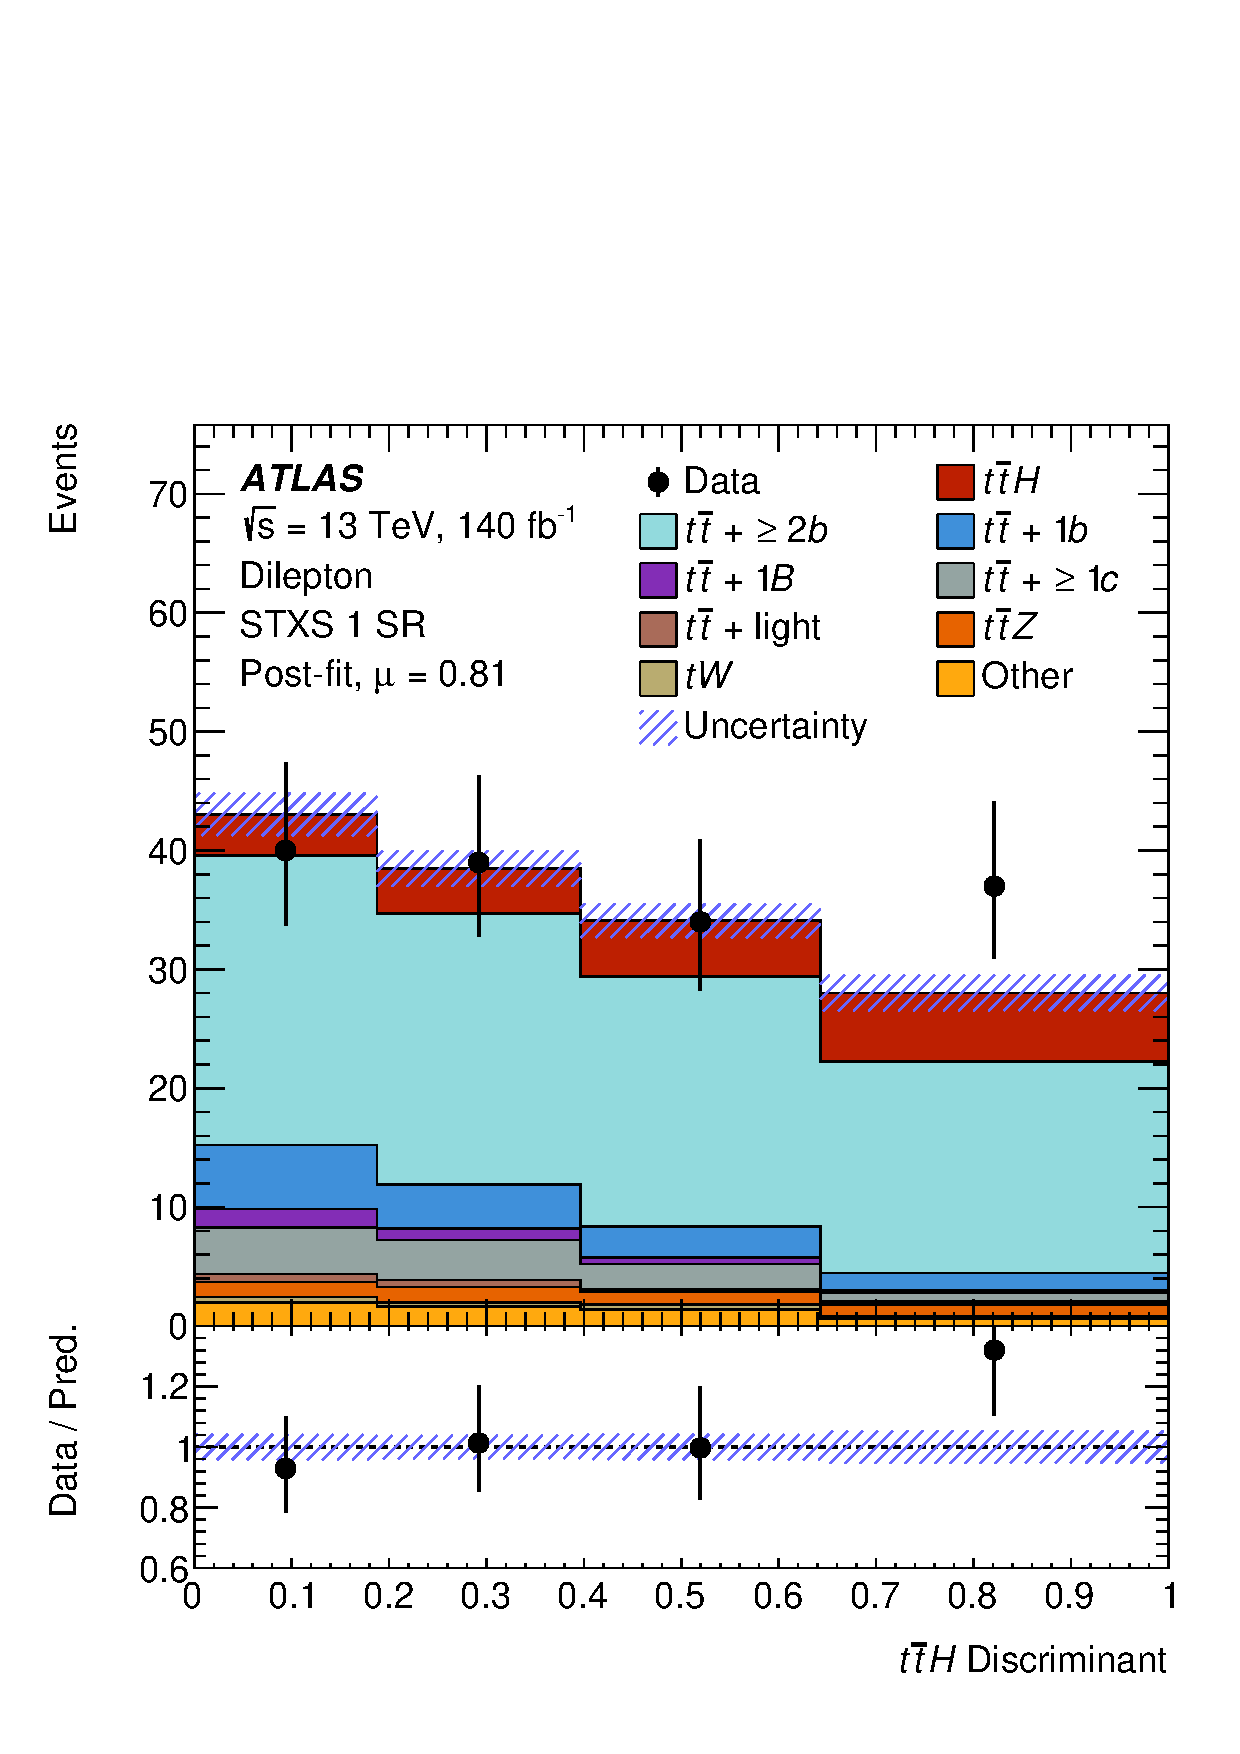
\includegraphics[width=\linewidth]{Section_tthbb_analysis/figures/Results/ttH_STXS1_2l_postFit.pdf}
        \caption{}
    \end{subfigure}
    \hfill
    \begin{subfigure}{0.3\textwidth}
        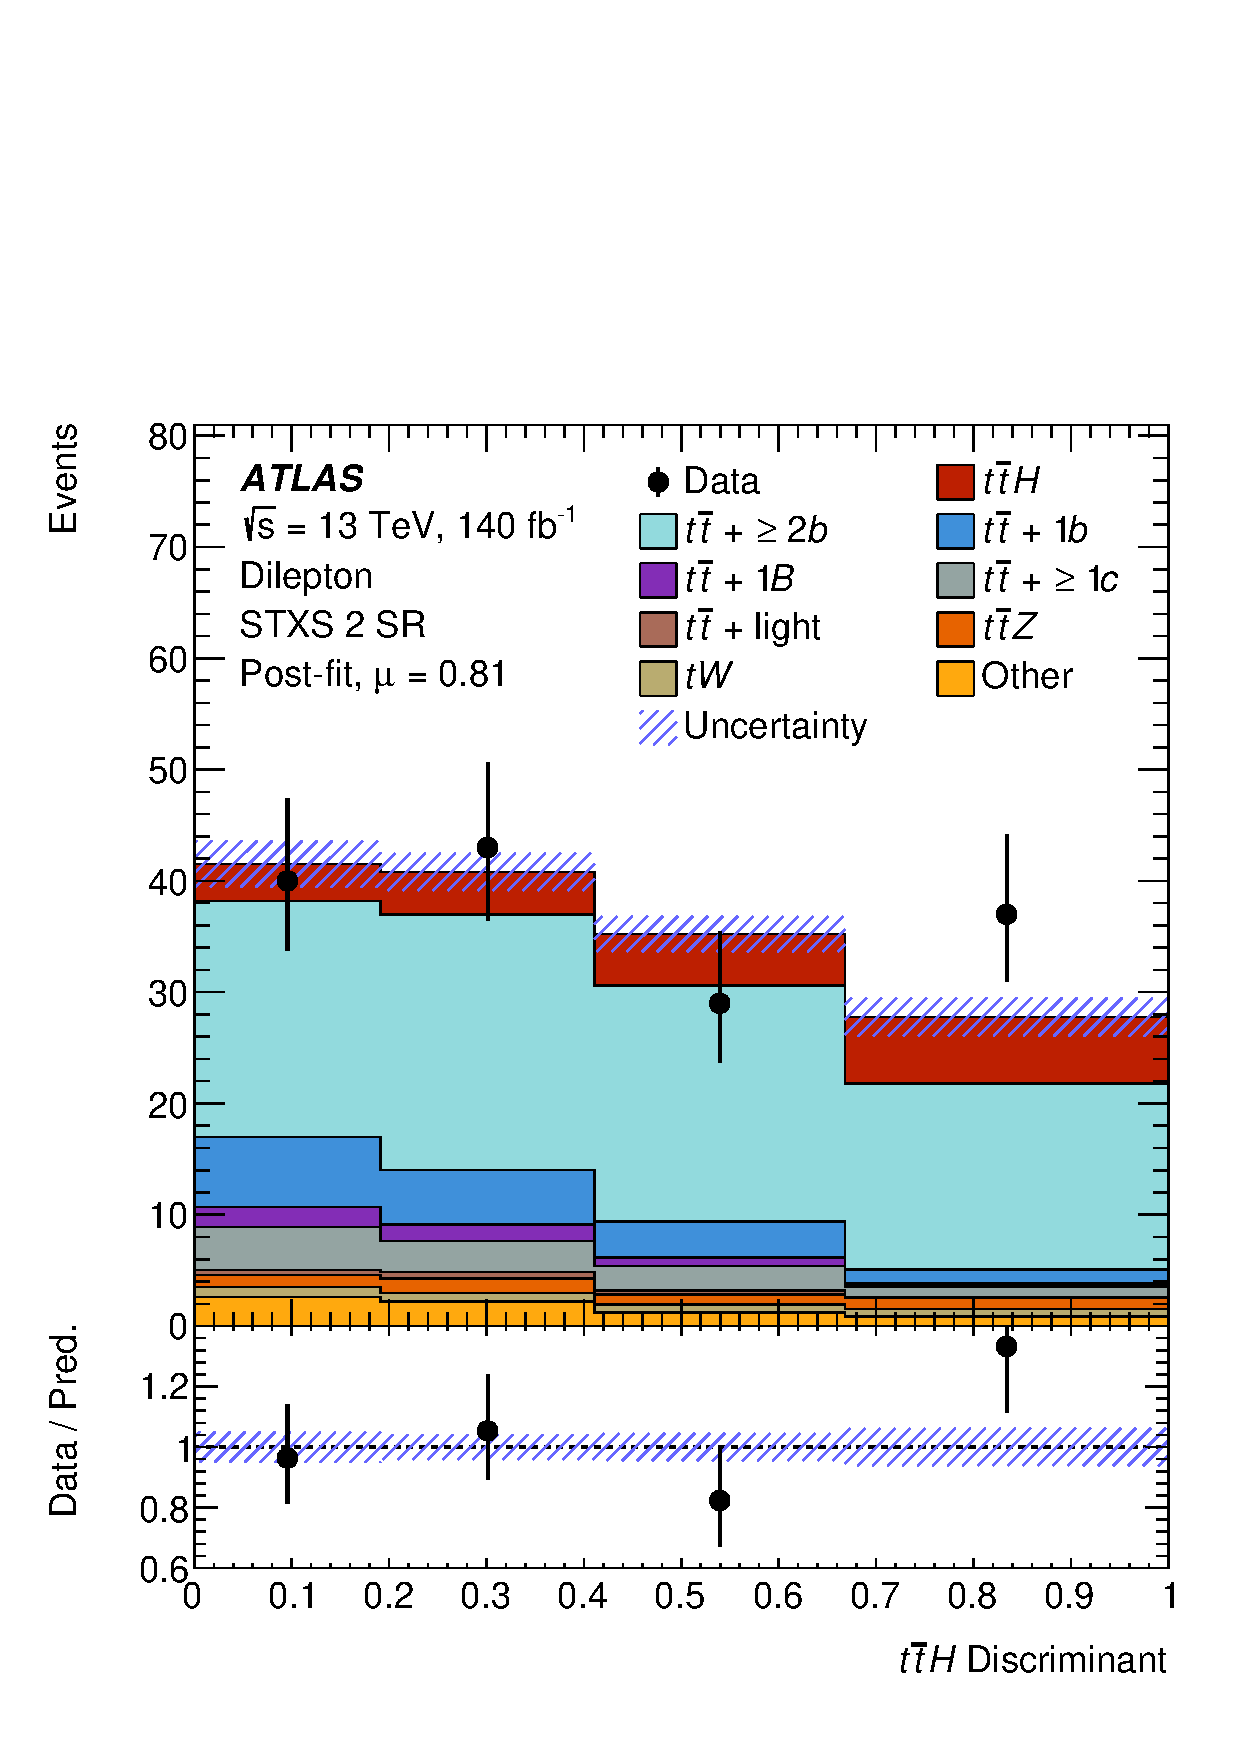
\includegraphics[width=\linewidth]{Section_tthbb_analysis/figures/Results/ttH_STXS2_2l_postFit.pdf}
        \caption{}
    \end{subfigure}
    \hfill
    \begin{subfigure}{0.3\textwidth}
        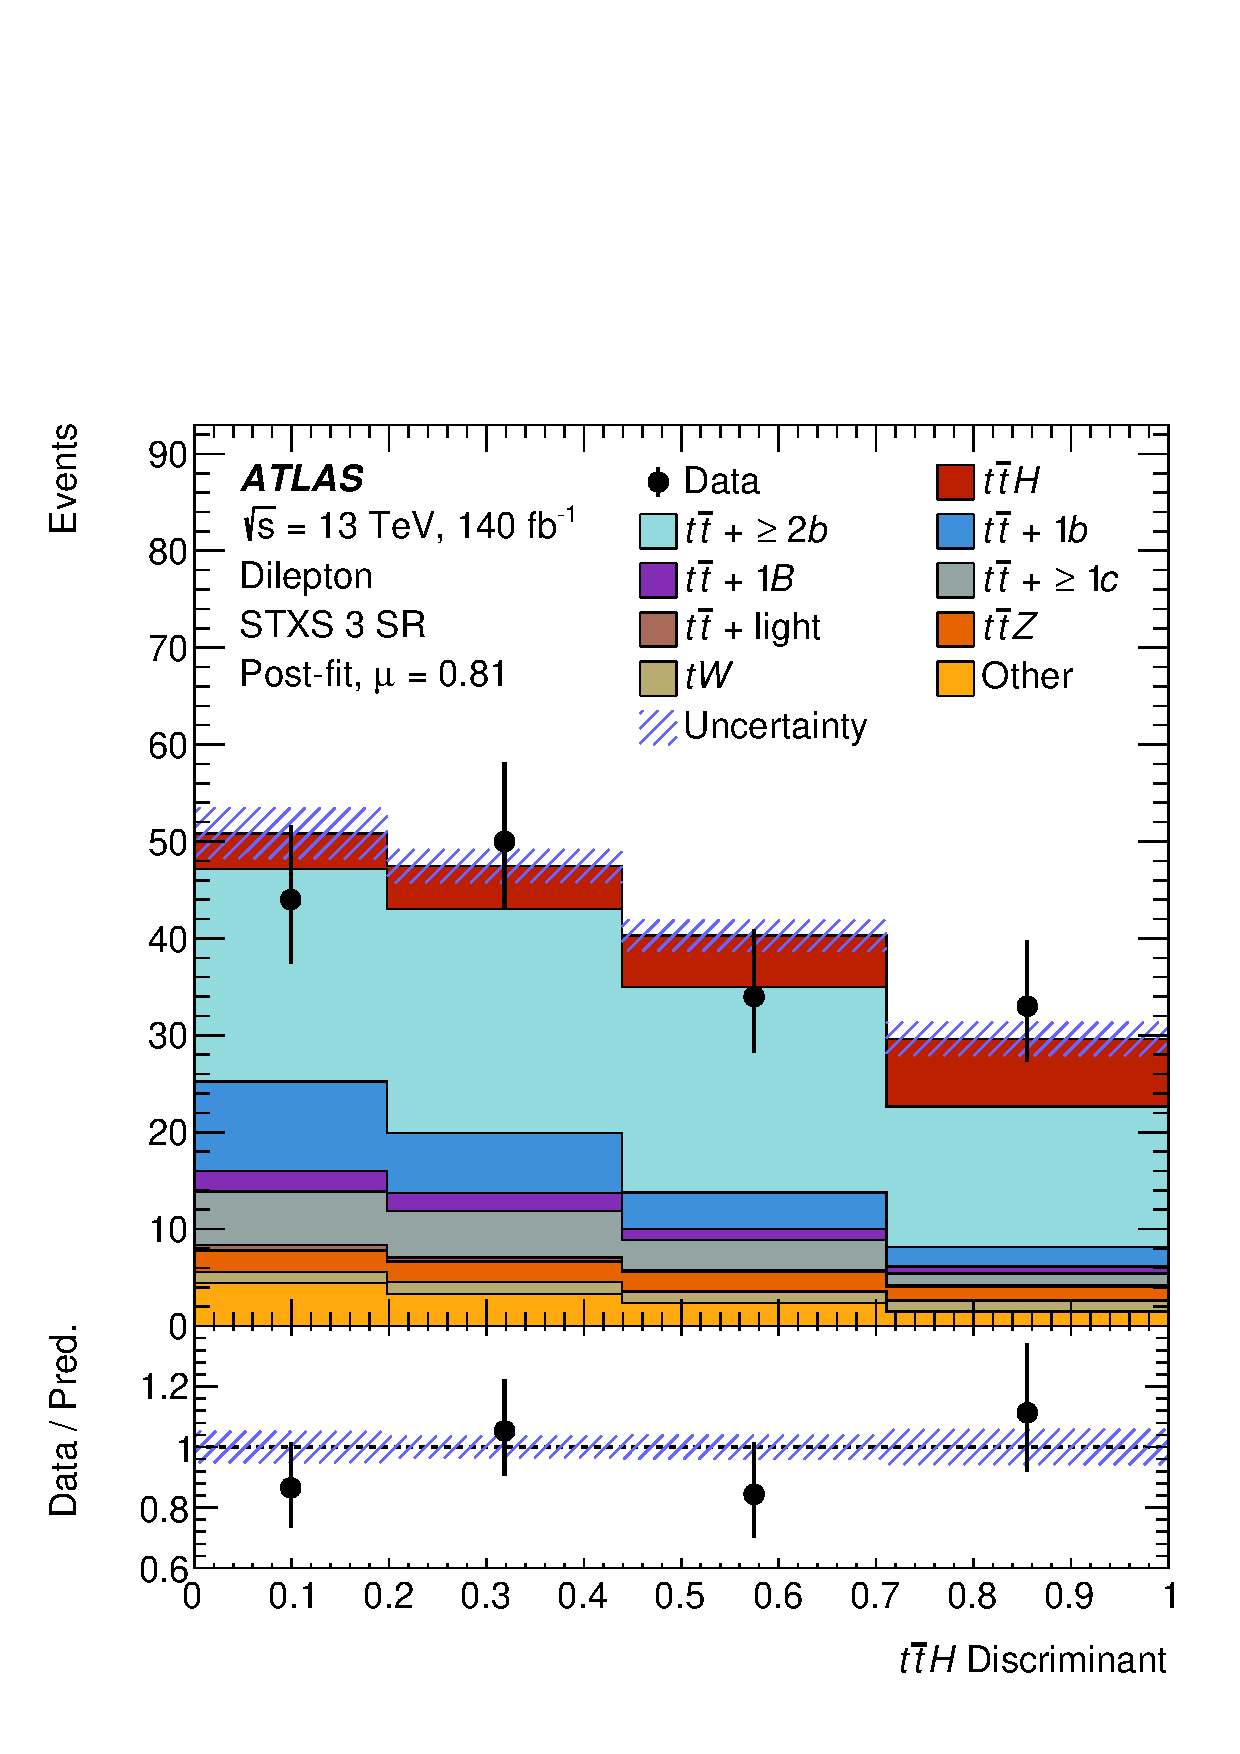
\includegraphics[width=\linewidth]{Section_tthbb_analysis/figures/Results/ttH_STXS3_2l_postFit.pdf}
        \caption{}
    \end{subfigure}
    
    \vspace{0.5cm} % space between rows
    
    % Row 2: 3 images
    \begin{subfigure}{0.3\textwidth}
        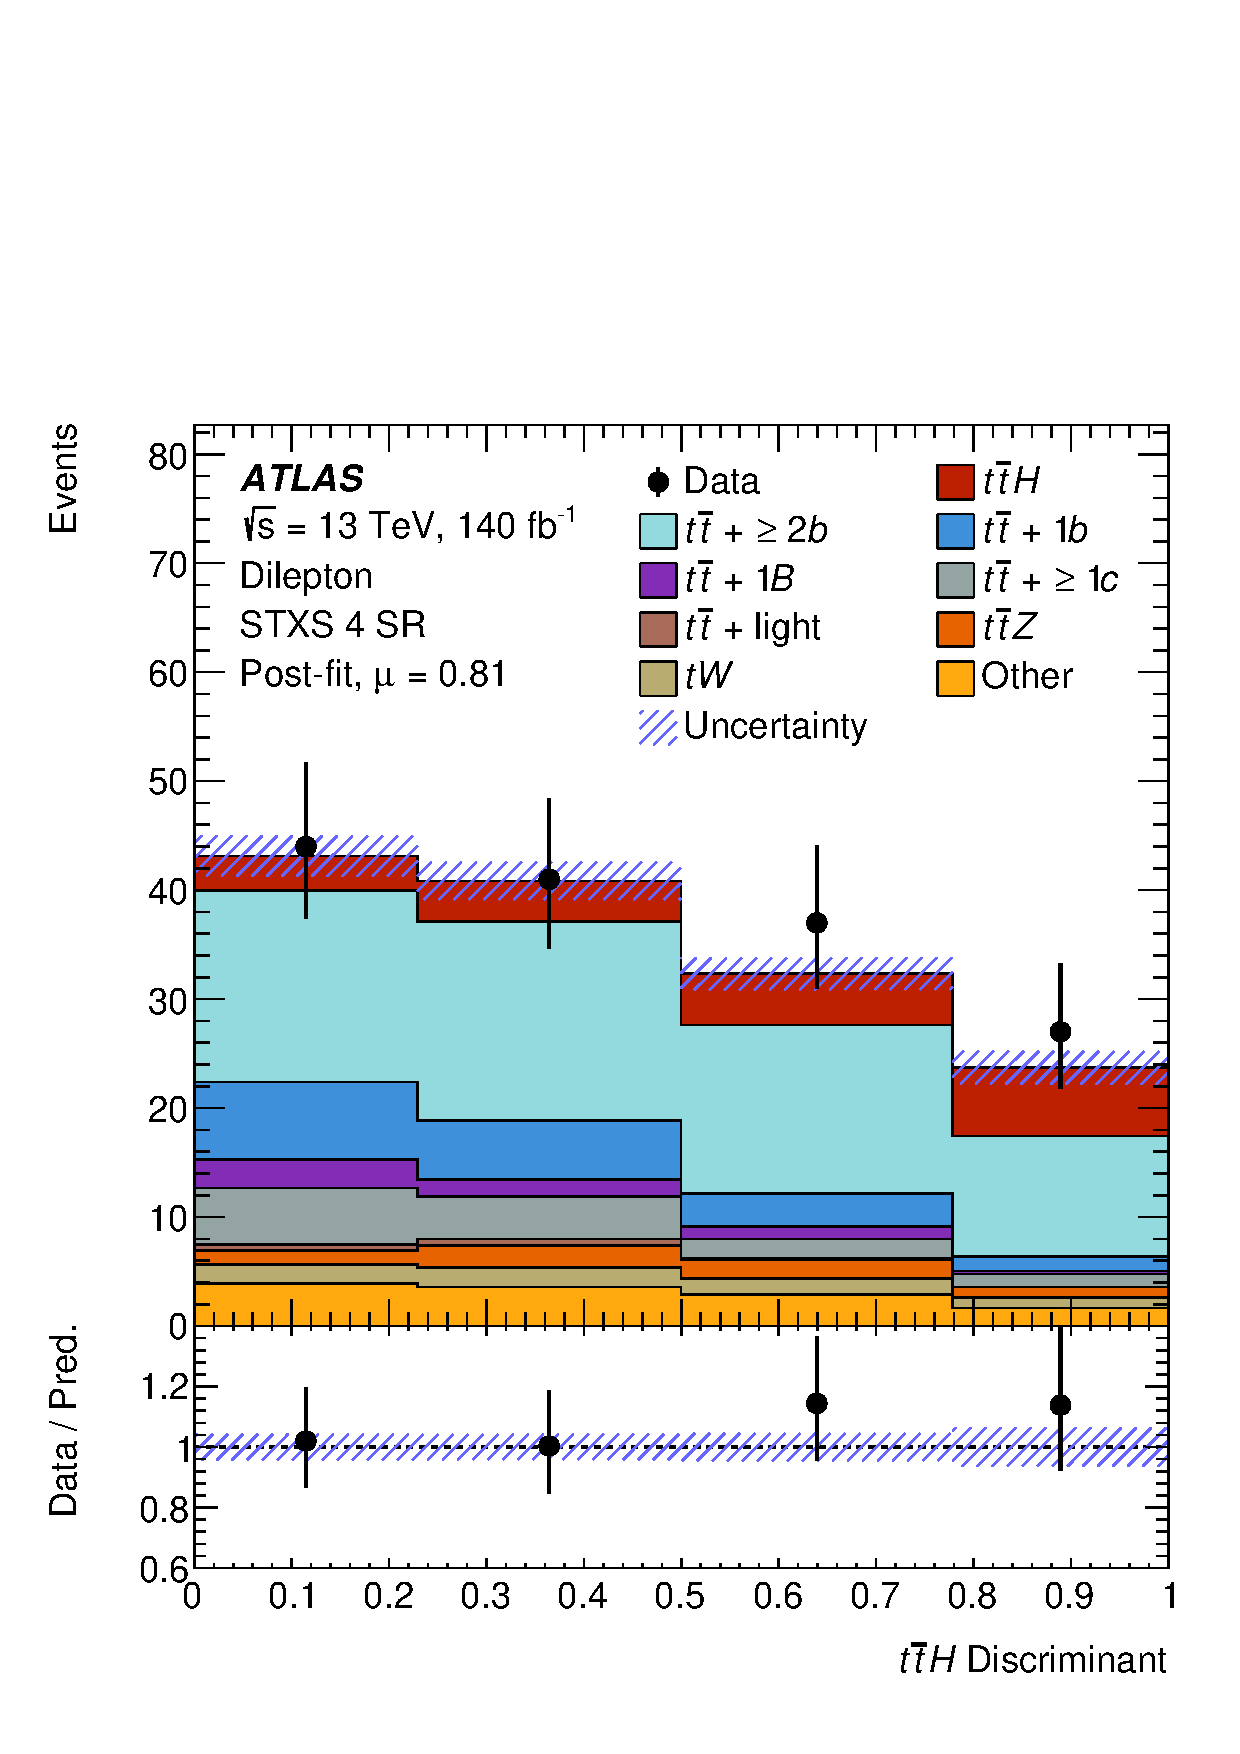
\includegraphics[width=\linewidth]{Section_tthbb_analysis/figures/Results/ttH_STXS4_2l_postFit.pdf}
        \caption{j}
    \end{subfigure}
    \hfill
    \begin{subfigure}{0.3\textwidth}
        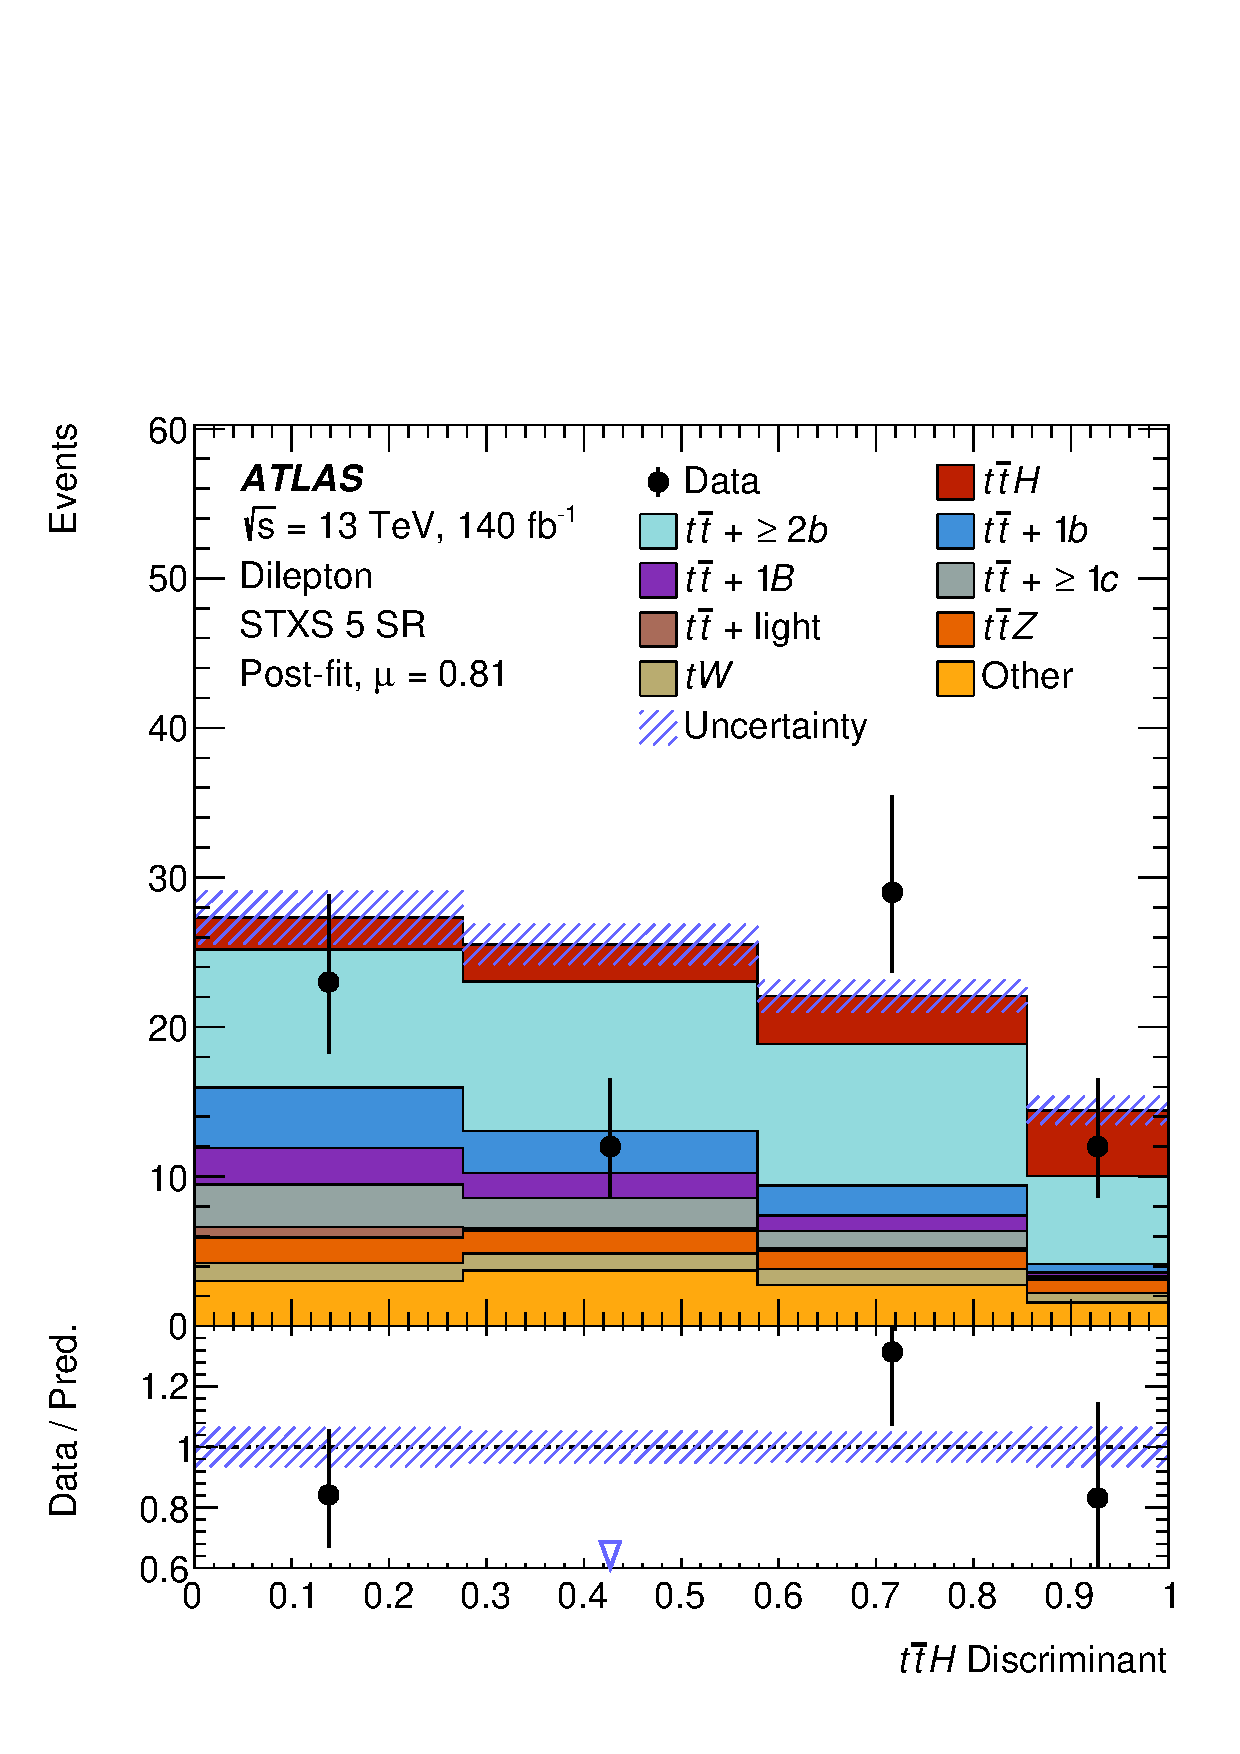
\includegraphics[width=\linewidth]{Section_tthbb_analysis/figures/Results/ttH_STXS5_2l_postFit.pdf}
        \caption{}
    \end{subfigure}
    \hfill
    \begin{subfigure}{0.3\textwidth}
        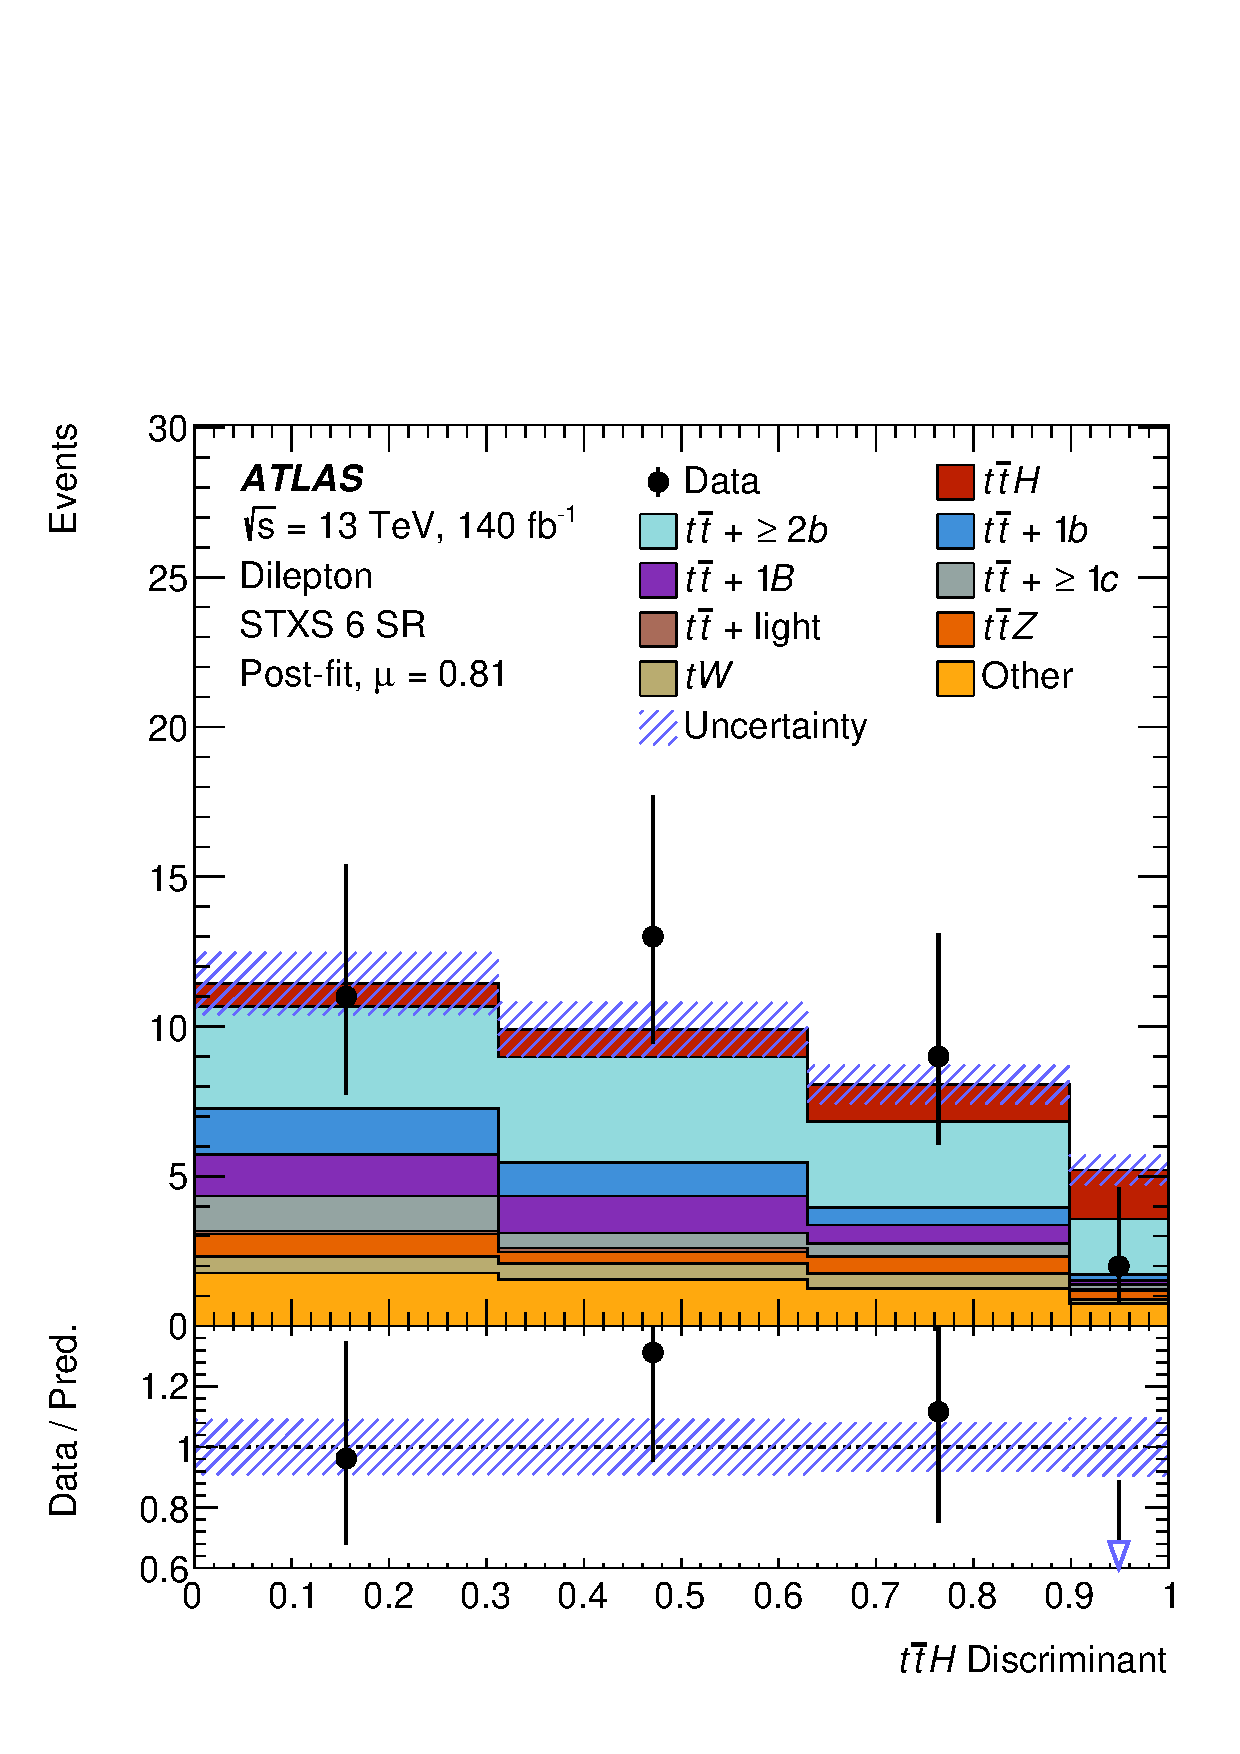
\includegraphics[width=\linewidth]{Section_tthbb_analysis/figures/Results/ttH_STXS6_2l_postFit.pdf}
        \caption{}
    \end{subfigure}

    
\caption{Post-fit distributions of the seven signal regions in the Di-lepton channel:  
(a) STXS 1,  
(b) STXS 2,  
(c) STXS 3,  
(d) STXS 4,  
(e) STXS 5,  
(f) STXS 6.}

    \label{fig:1l_data_mc_pre_fit_SR}
\end{figure}
\begin{figure}[!htb]
    \centering
    % Row 1: 3 images
    \begin{subfigure}{0.3\textwidth}
        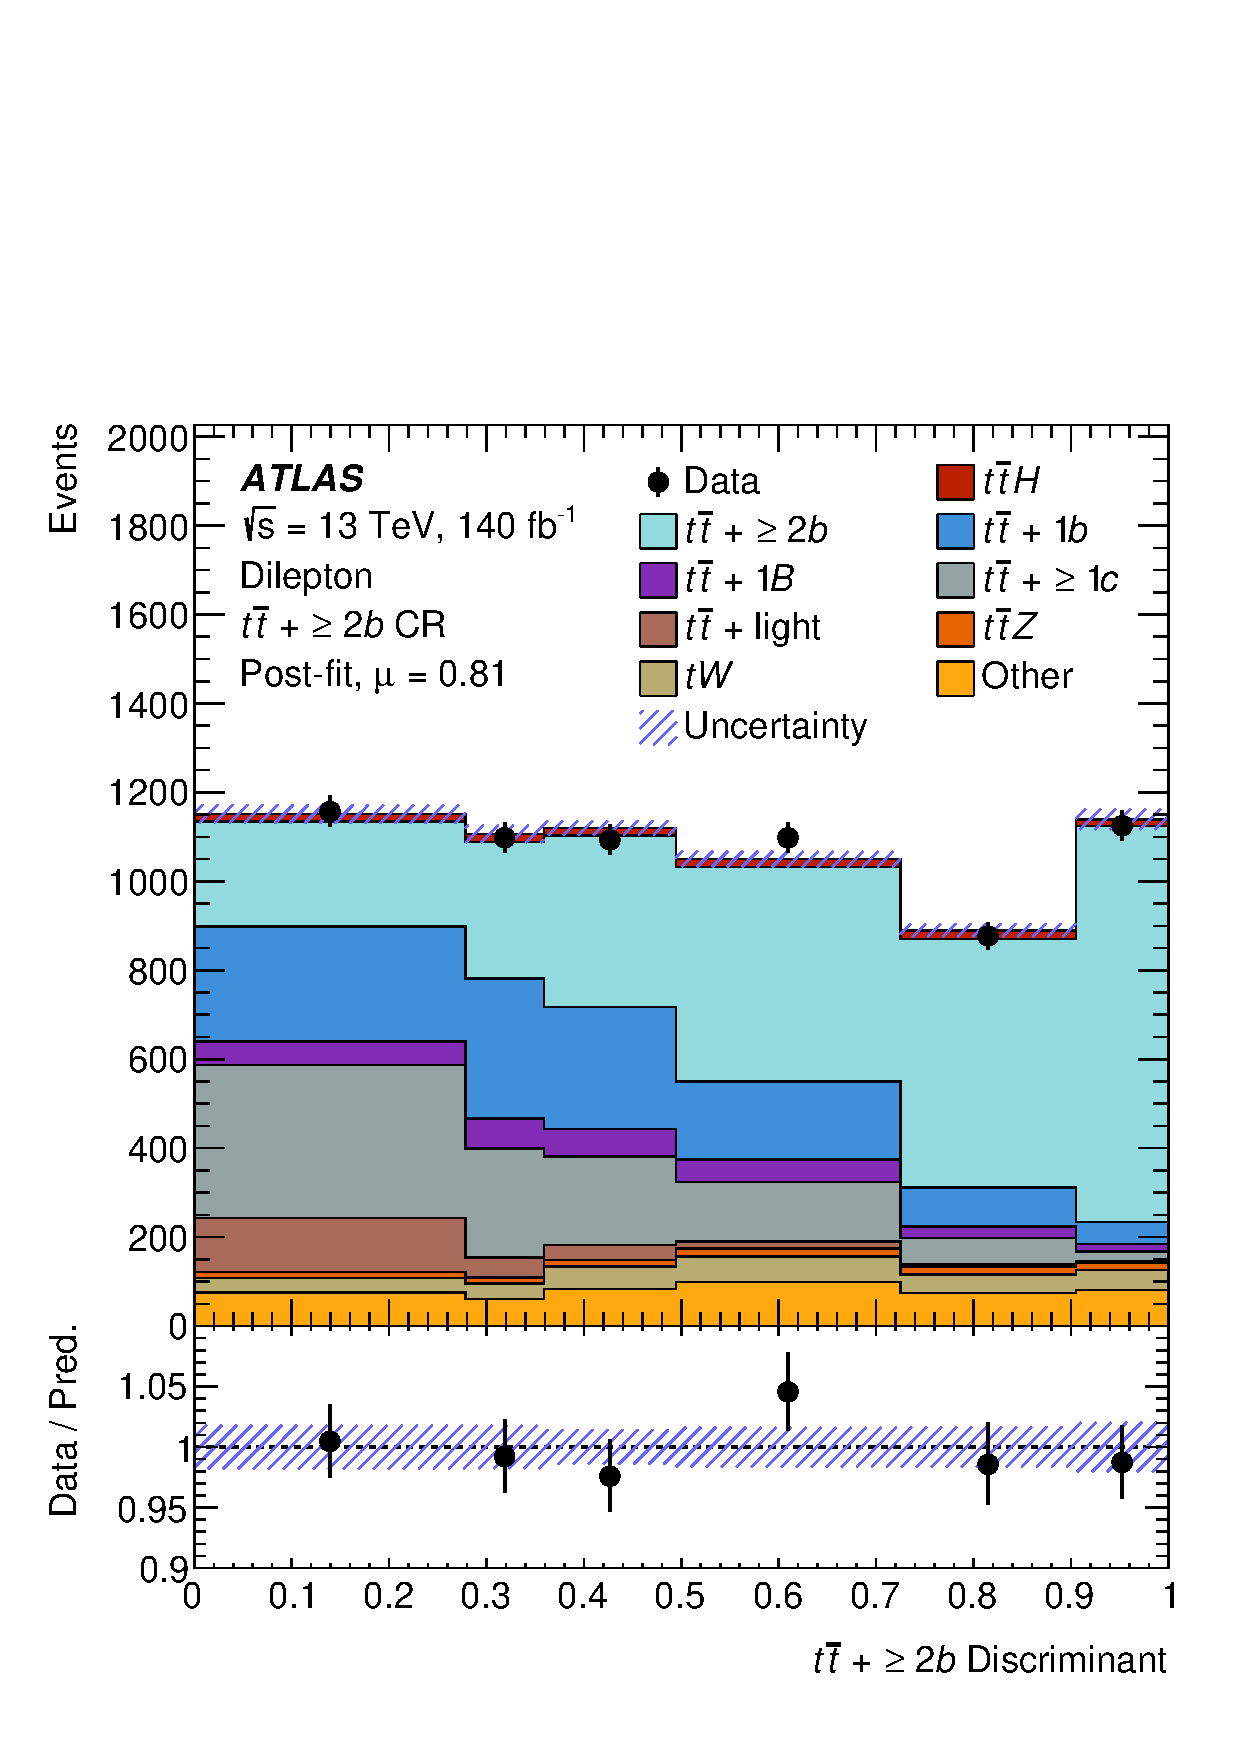
\includegraphics[width=\linewidth]{Section_tthbb_analysis/figures/Results/tt2b_2l_postFit.pdf}
        \caption{}
    \end{subfigure}
\hfill
    \begin{subfigure}{0.3\textwidth}
        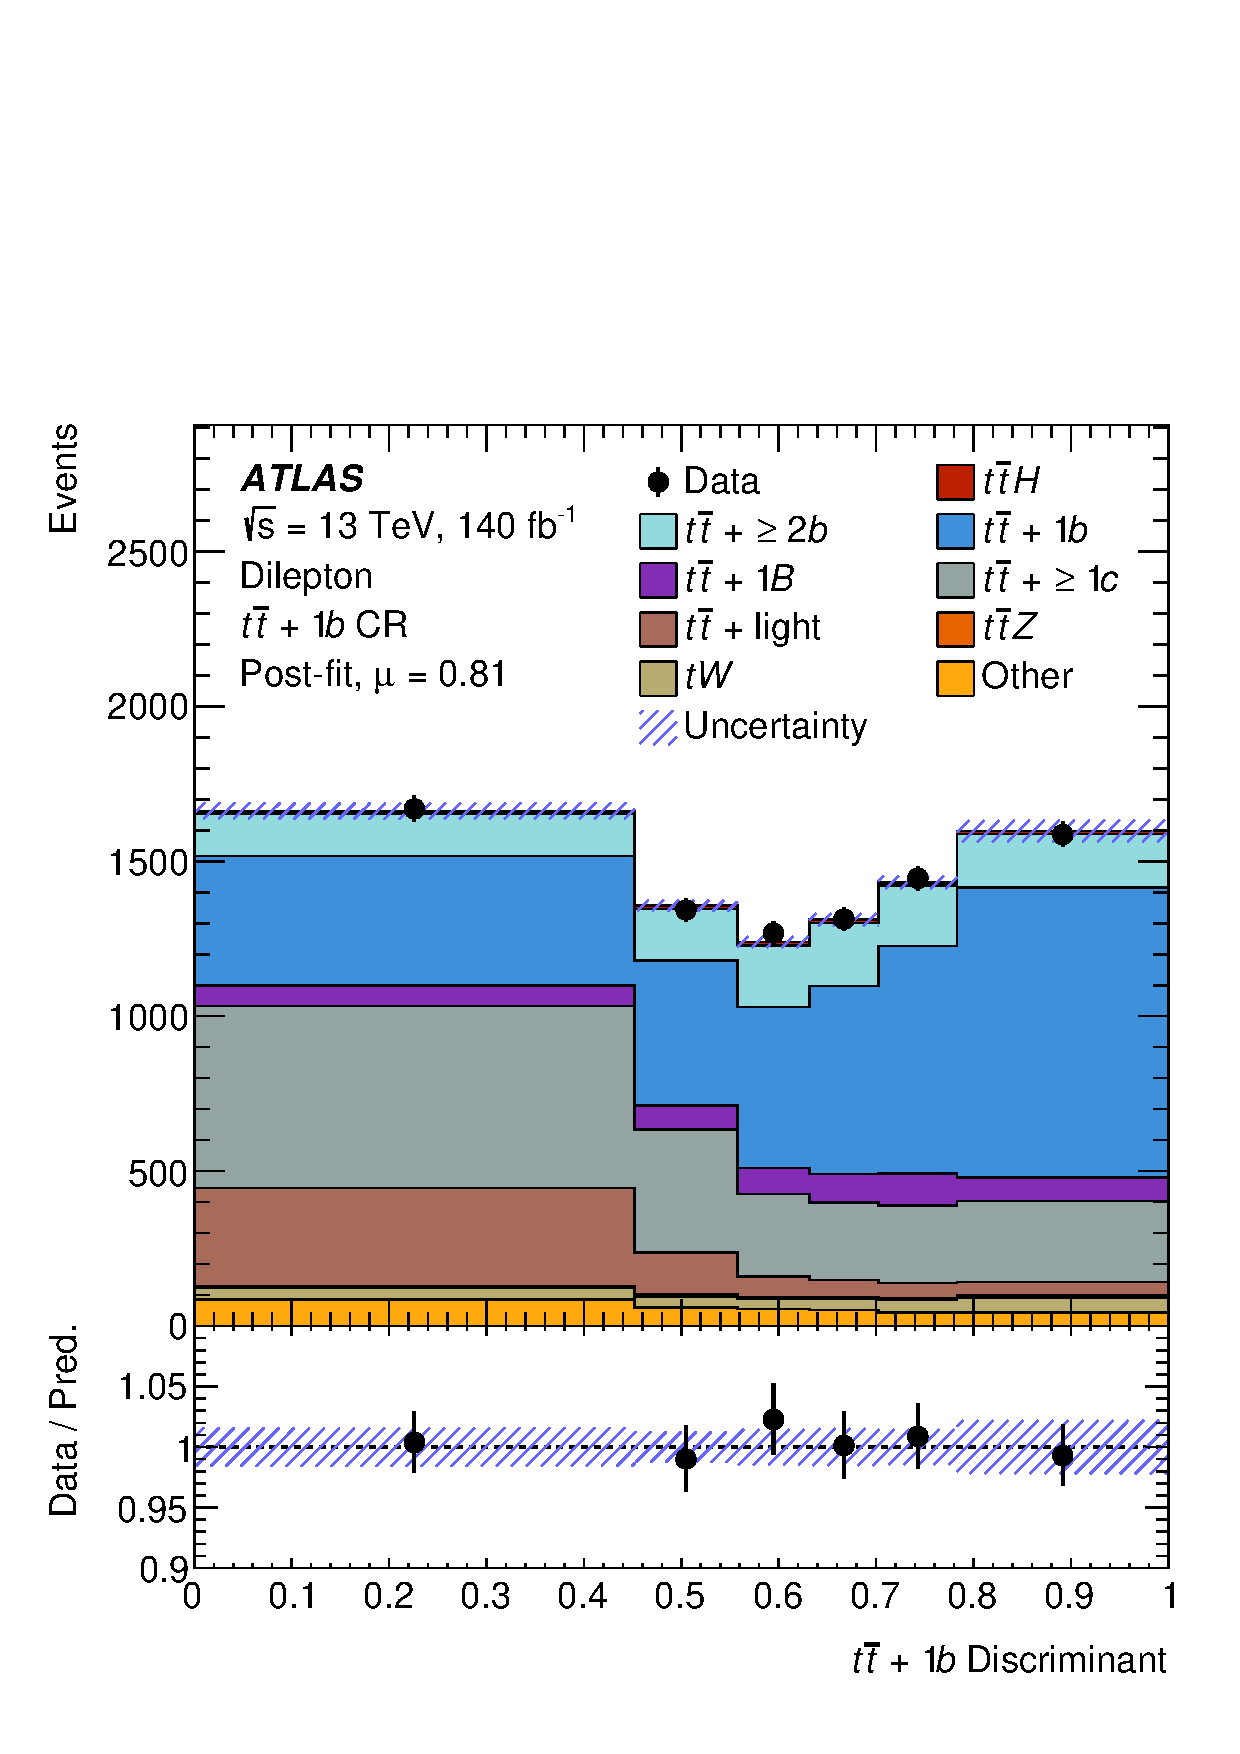
\includegraphics[width=\linewidth]{Section_tthbb_analysis/figures/Results/tt1b_2l_postFit.pdf}
        \caption{j}
    \end{subfigure}
    \hfill
    \begin{subfigure}{0.3\textwidth}
        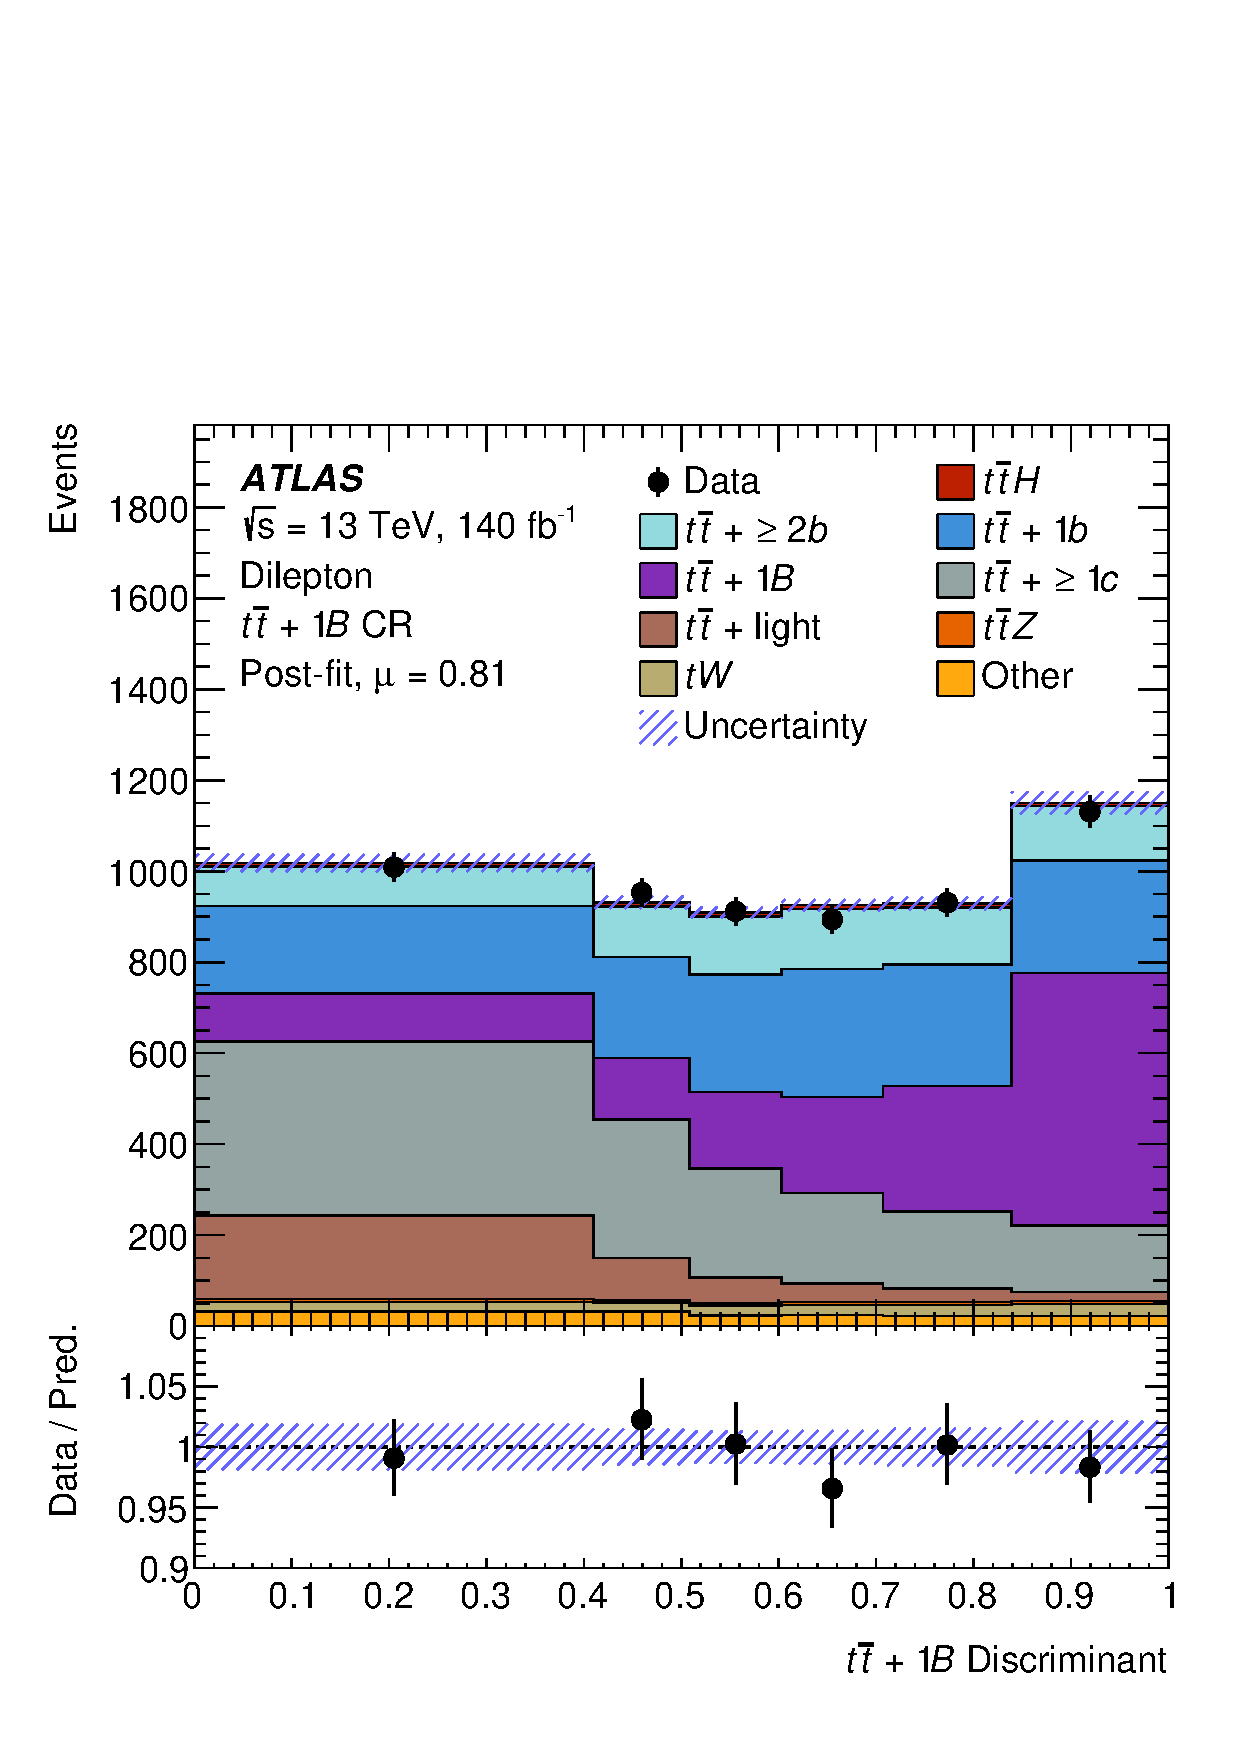
\includegraphics[width=\linewidth]{Section_tthbb_analysis/figures/Results/ttB_2l_postFit.pdf}
        \caption{}
    \end{subfigure}
    \vspace{0.5cm}
    \begin{subfigure}{0.3\textwidth}
        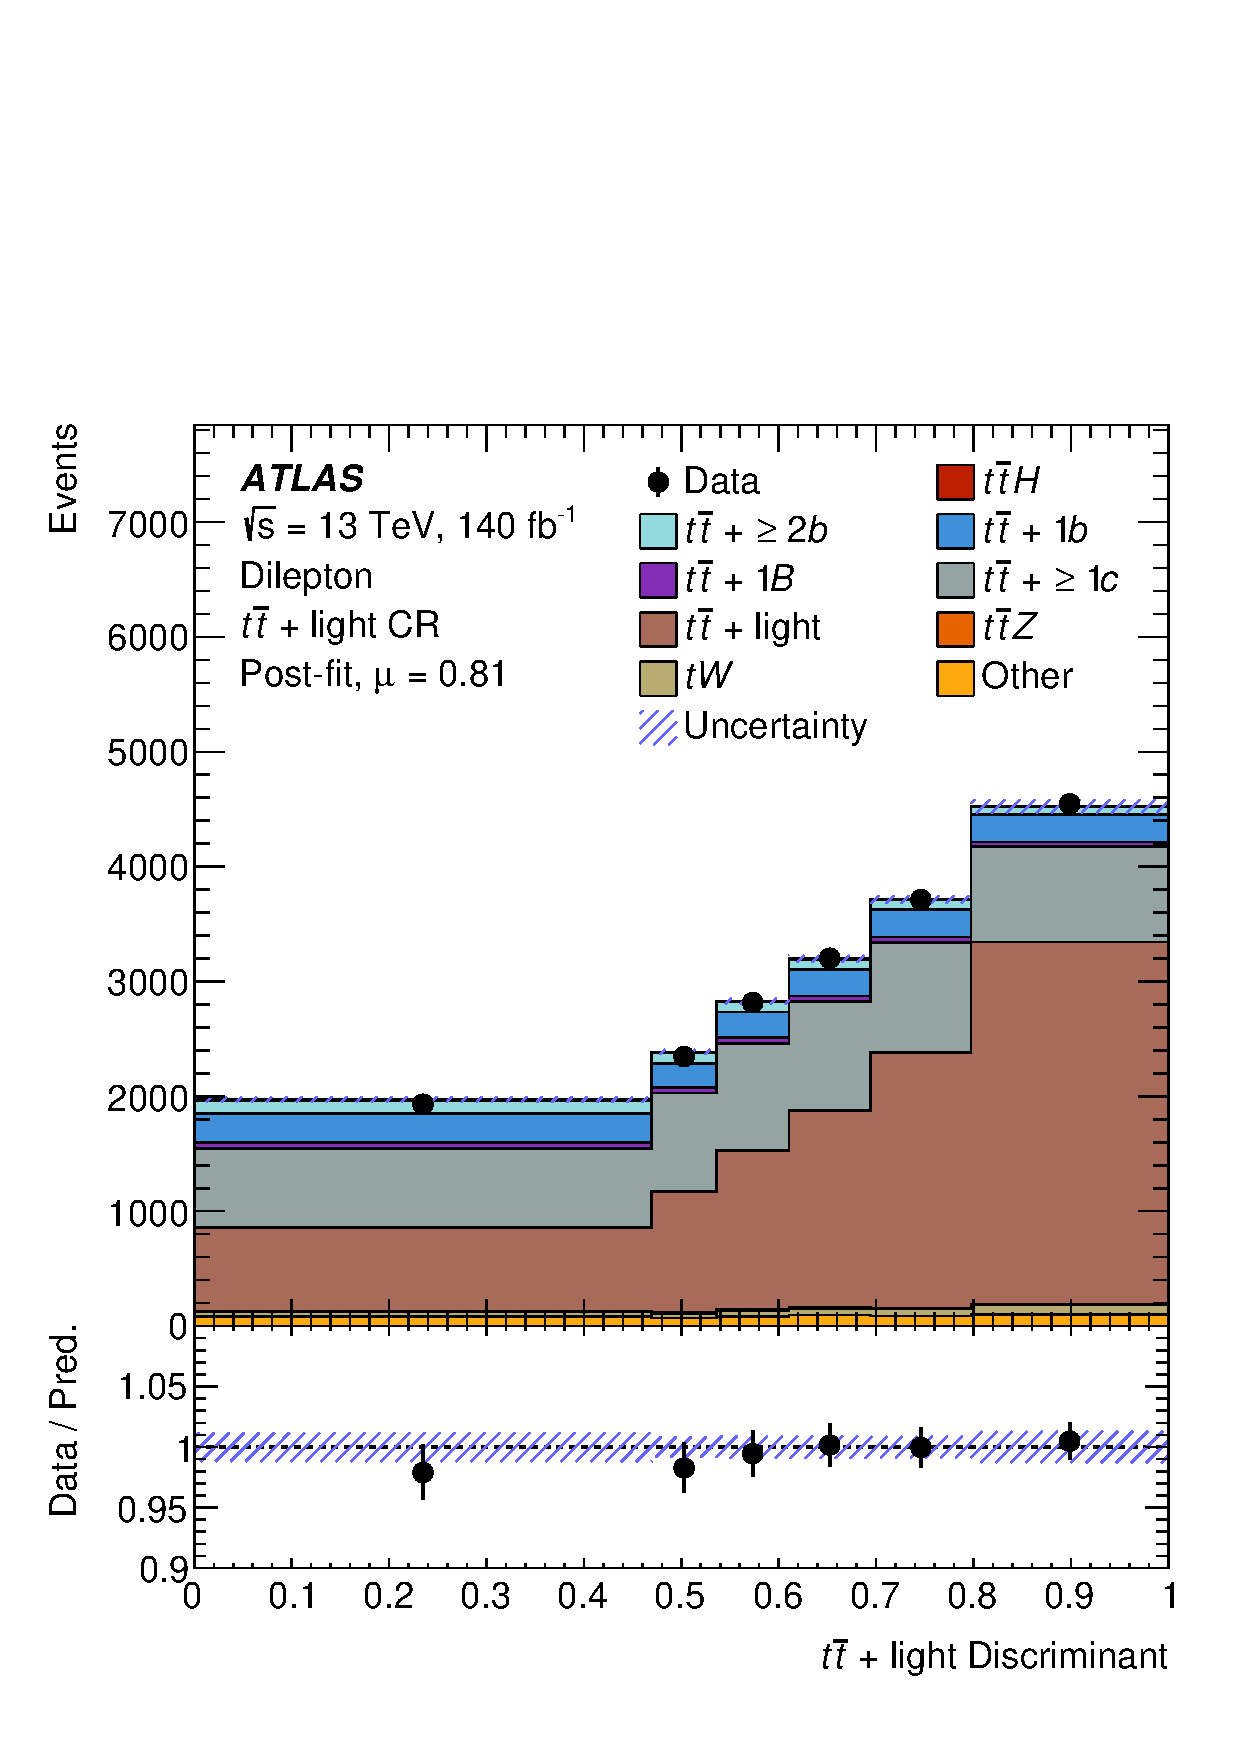
\includegraphics[width=\linewidth]{Section_tthbb_analysis/figures/Results/tt_light_2l_postFit.pdf}
        \caption{}
    \end{subfigure}
\hspace{0.1\textwidth}
    \begin{subfigure}{0.3\textwidth}
        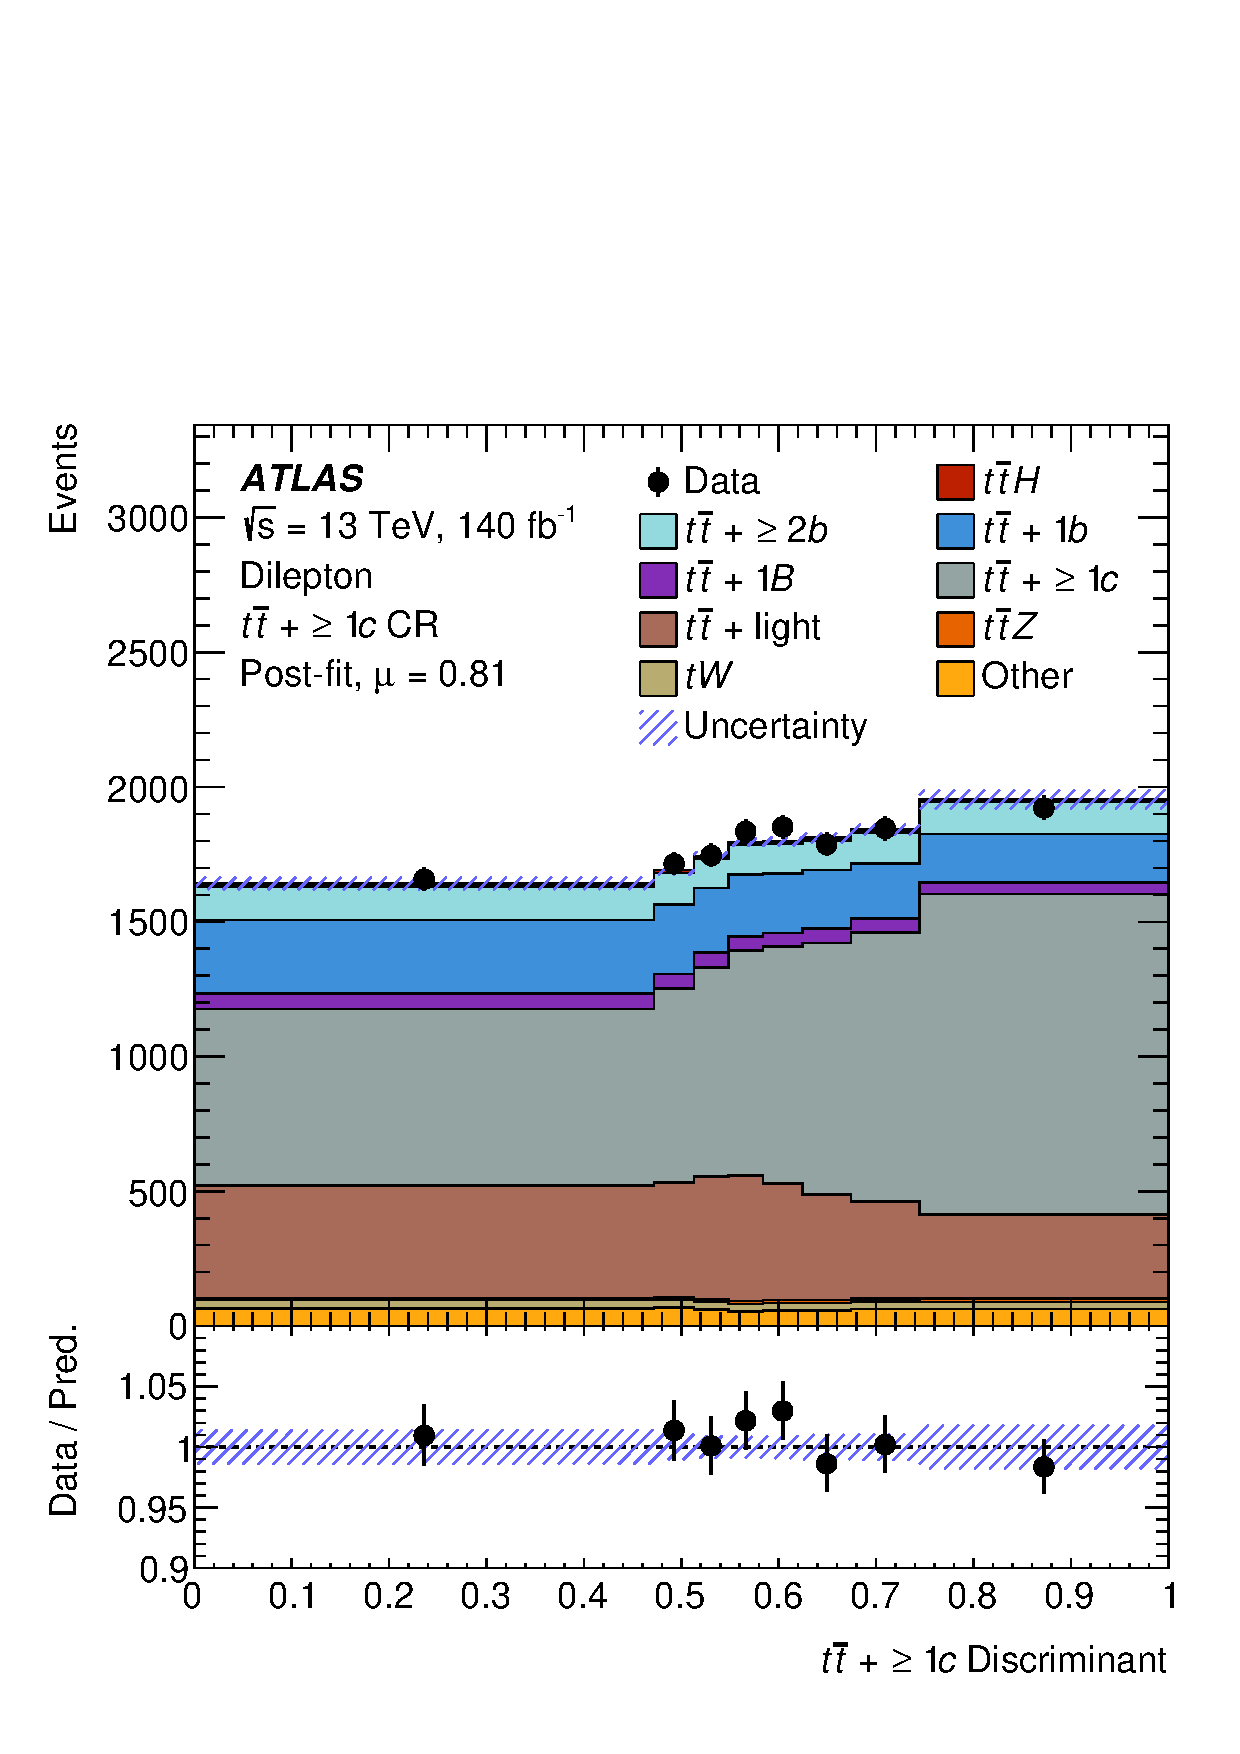
\includegraphics[width=\linewidth]{Section_tthbb_analysis/figures/Results/ttc_2l_postFit.pdf}
        \caption{}
    \end{subfigure}

    
    \caption{Post-fit distributions of the six control regions in the di-lepton channel: (a) $t\bar{t}+\geq 2b$, (b) $t\bar{t}+1b$, (c) $t\bar{t}+1B$, (d) $t\bar{t}+$light, (e) $t\bar{t}+\geq 1c$.}
    \label{fig:2l_data_mc_post_fit_CR}
\end{figure}
\section{STXS Ranking Plots}
\begin{figure}[!htb]
    \centering
    % Row 1: 3 images
    \begin{subfigure}{0.3\textwidth}
        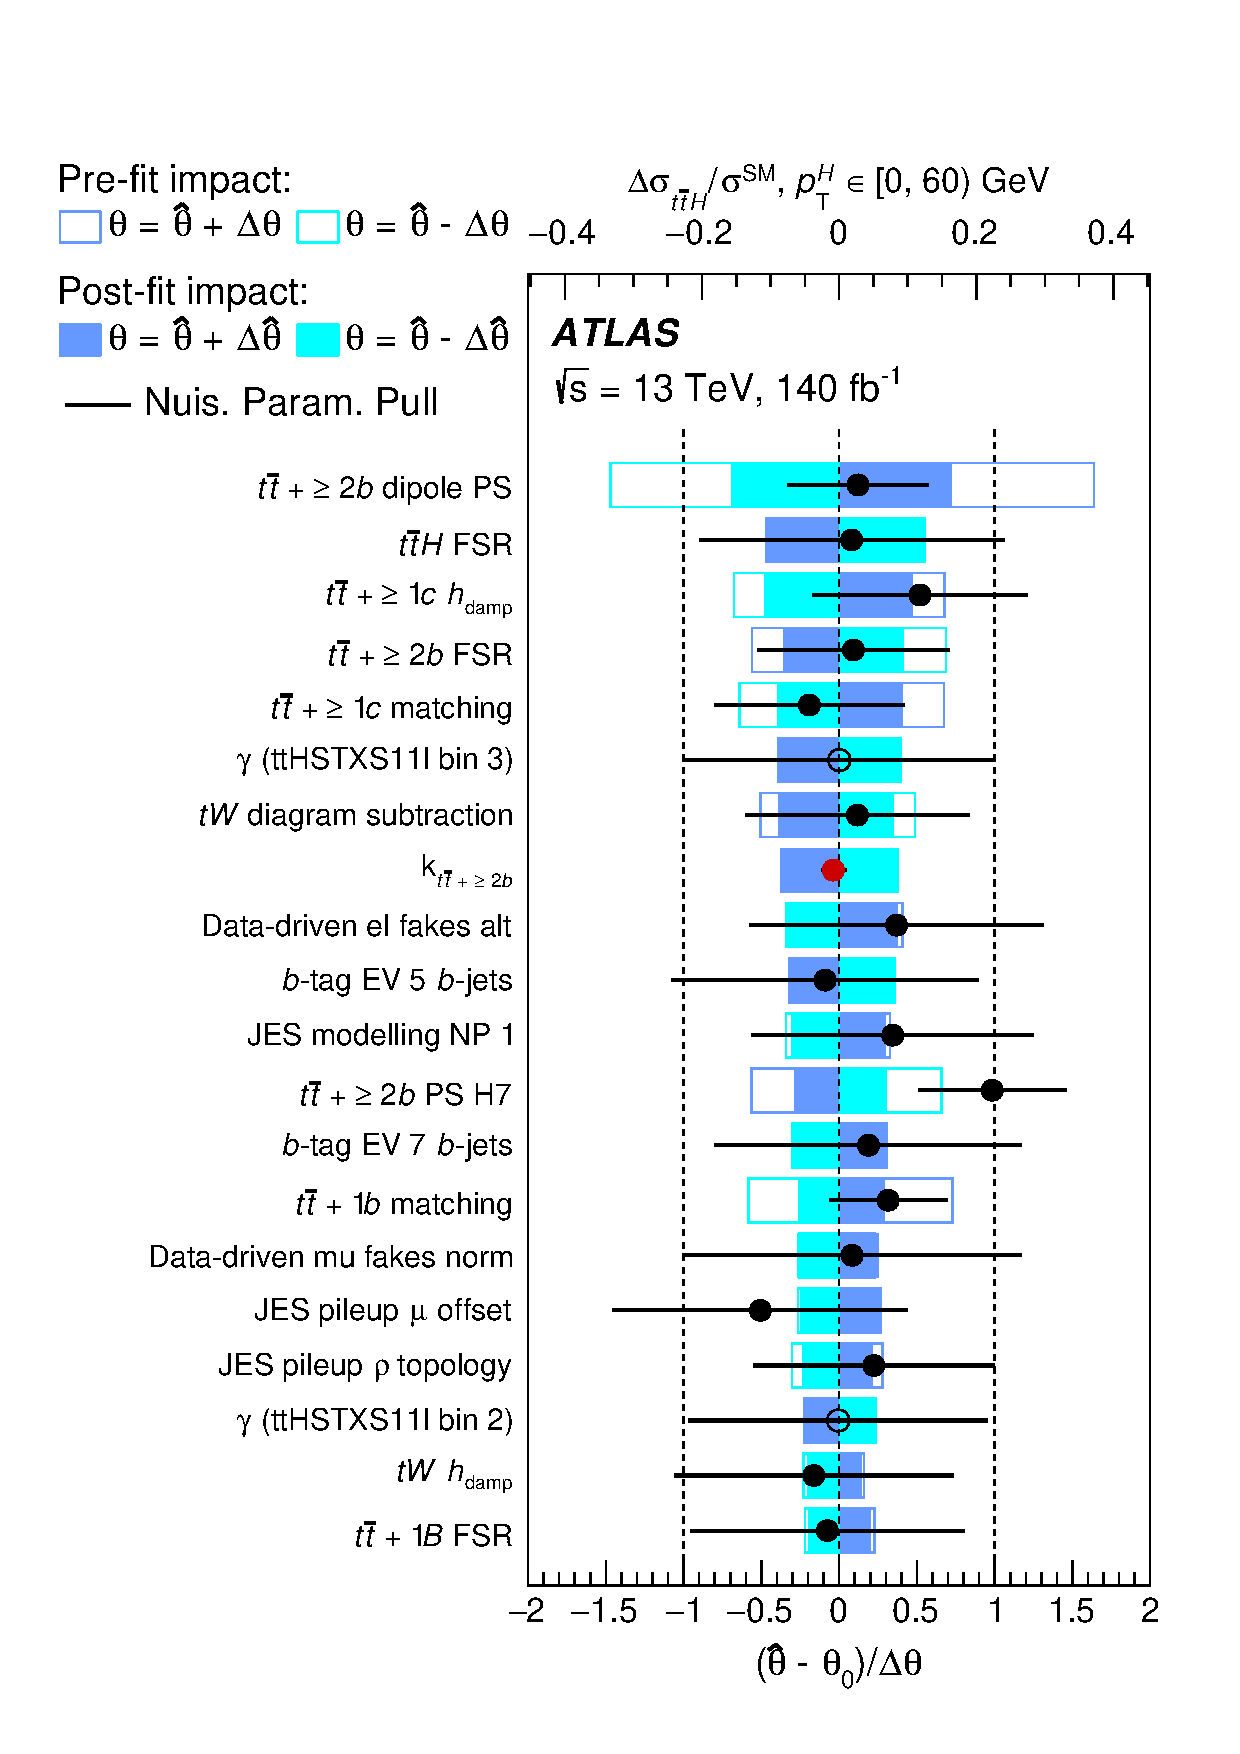
\includegraphics[width=\linewidth]{Section_tthbb_analysis/figures/Results/Ranking_ttH_ptH_0_60.pdf}
        \caption{}
    \end{subfigure}
    \hfill
    \begin{subfigure}{0.3\textwidth}
        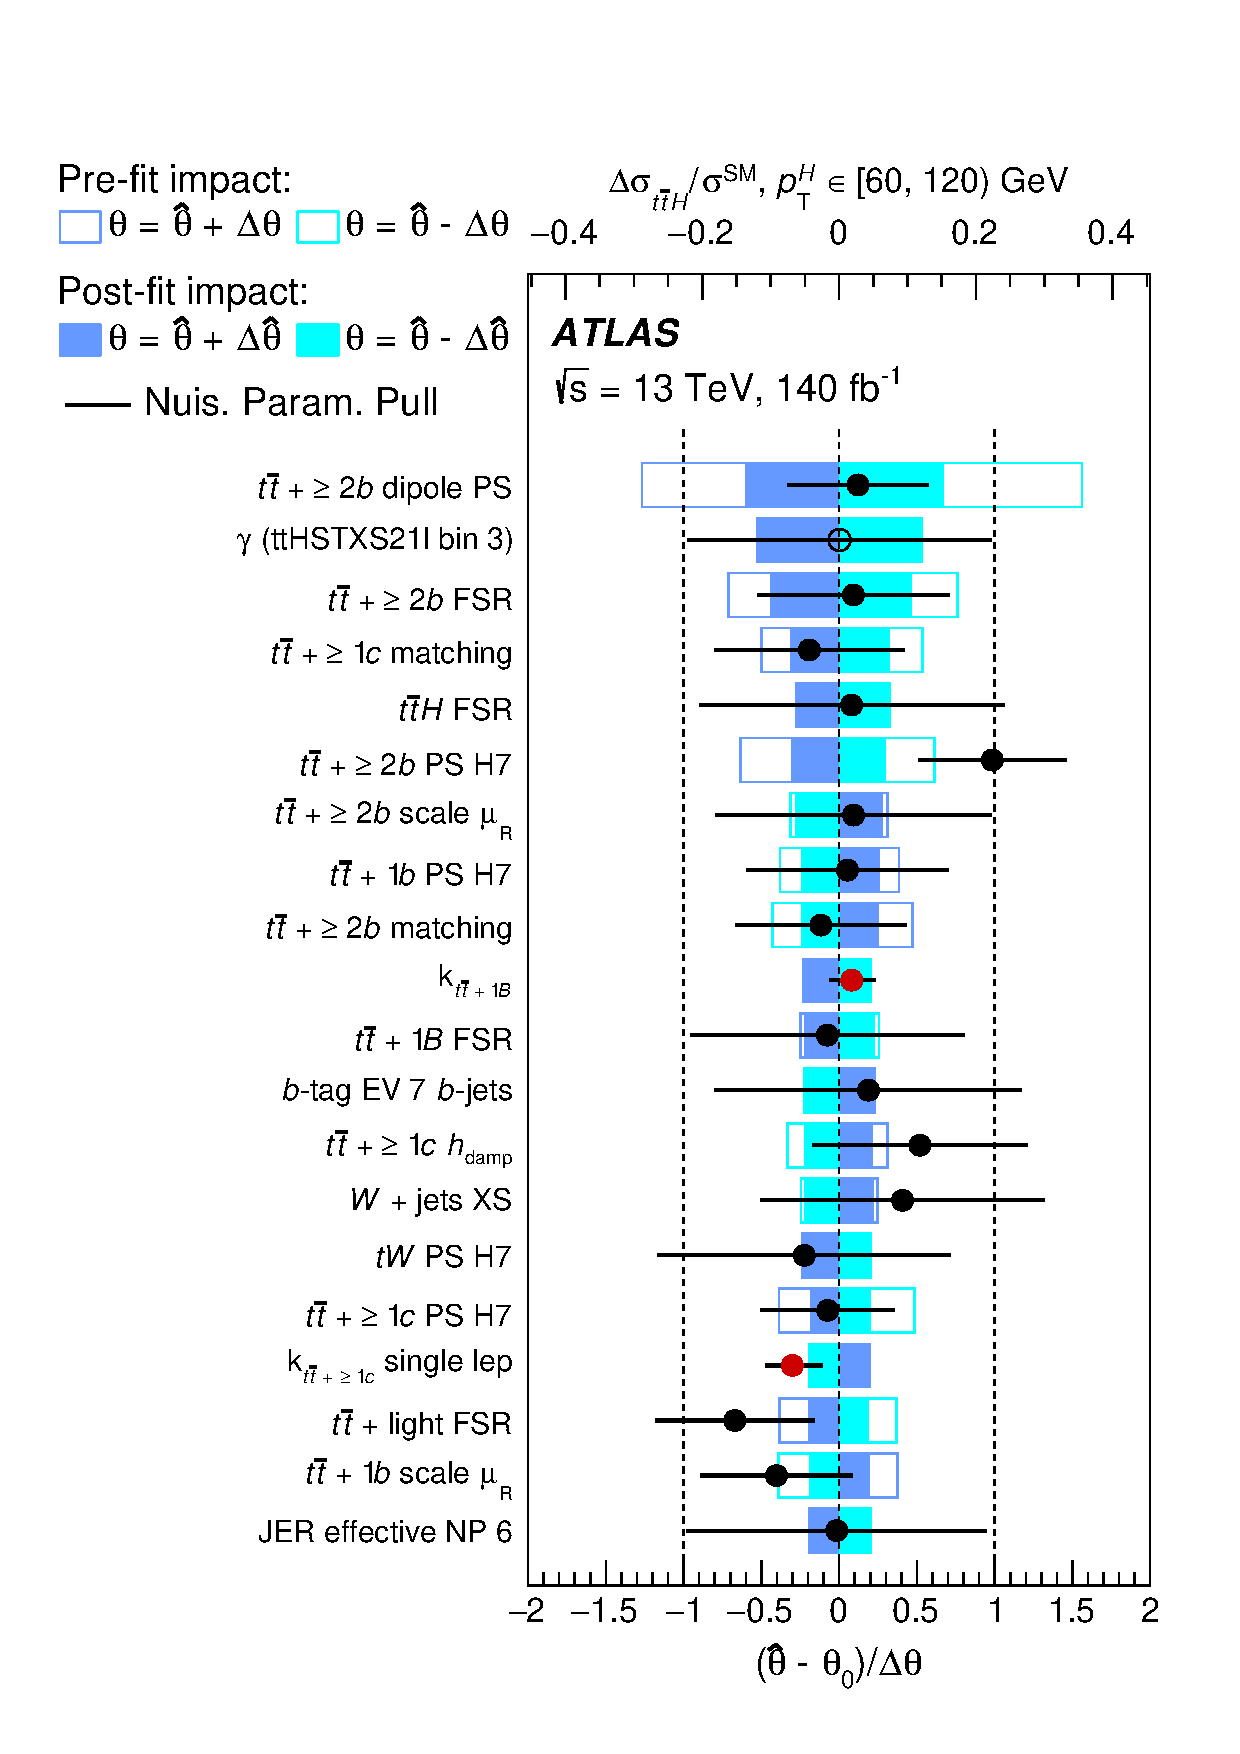
\includegraphics[width=\linewidth]{Section_tthbb_analysis/figures/Results/Ranking_ttH_ptH_60_120.pdf}
        \caption{}
    \end{subfigure}
    \hfill
    \begin{subfigure}{0.3\textwidth}
        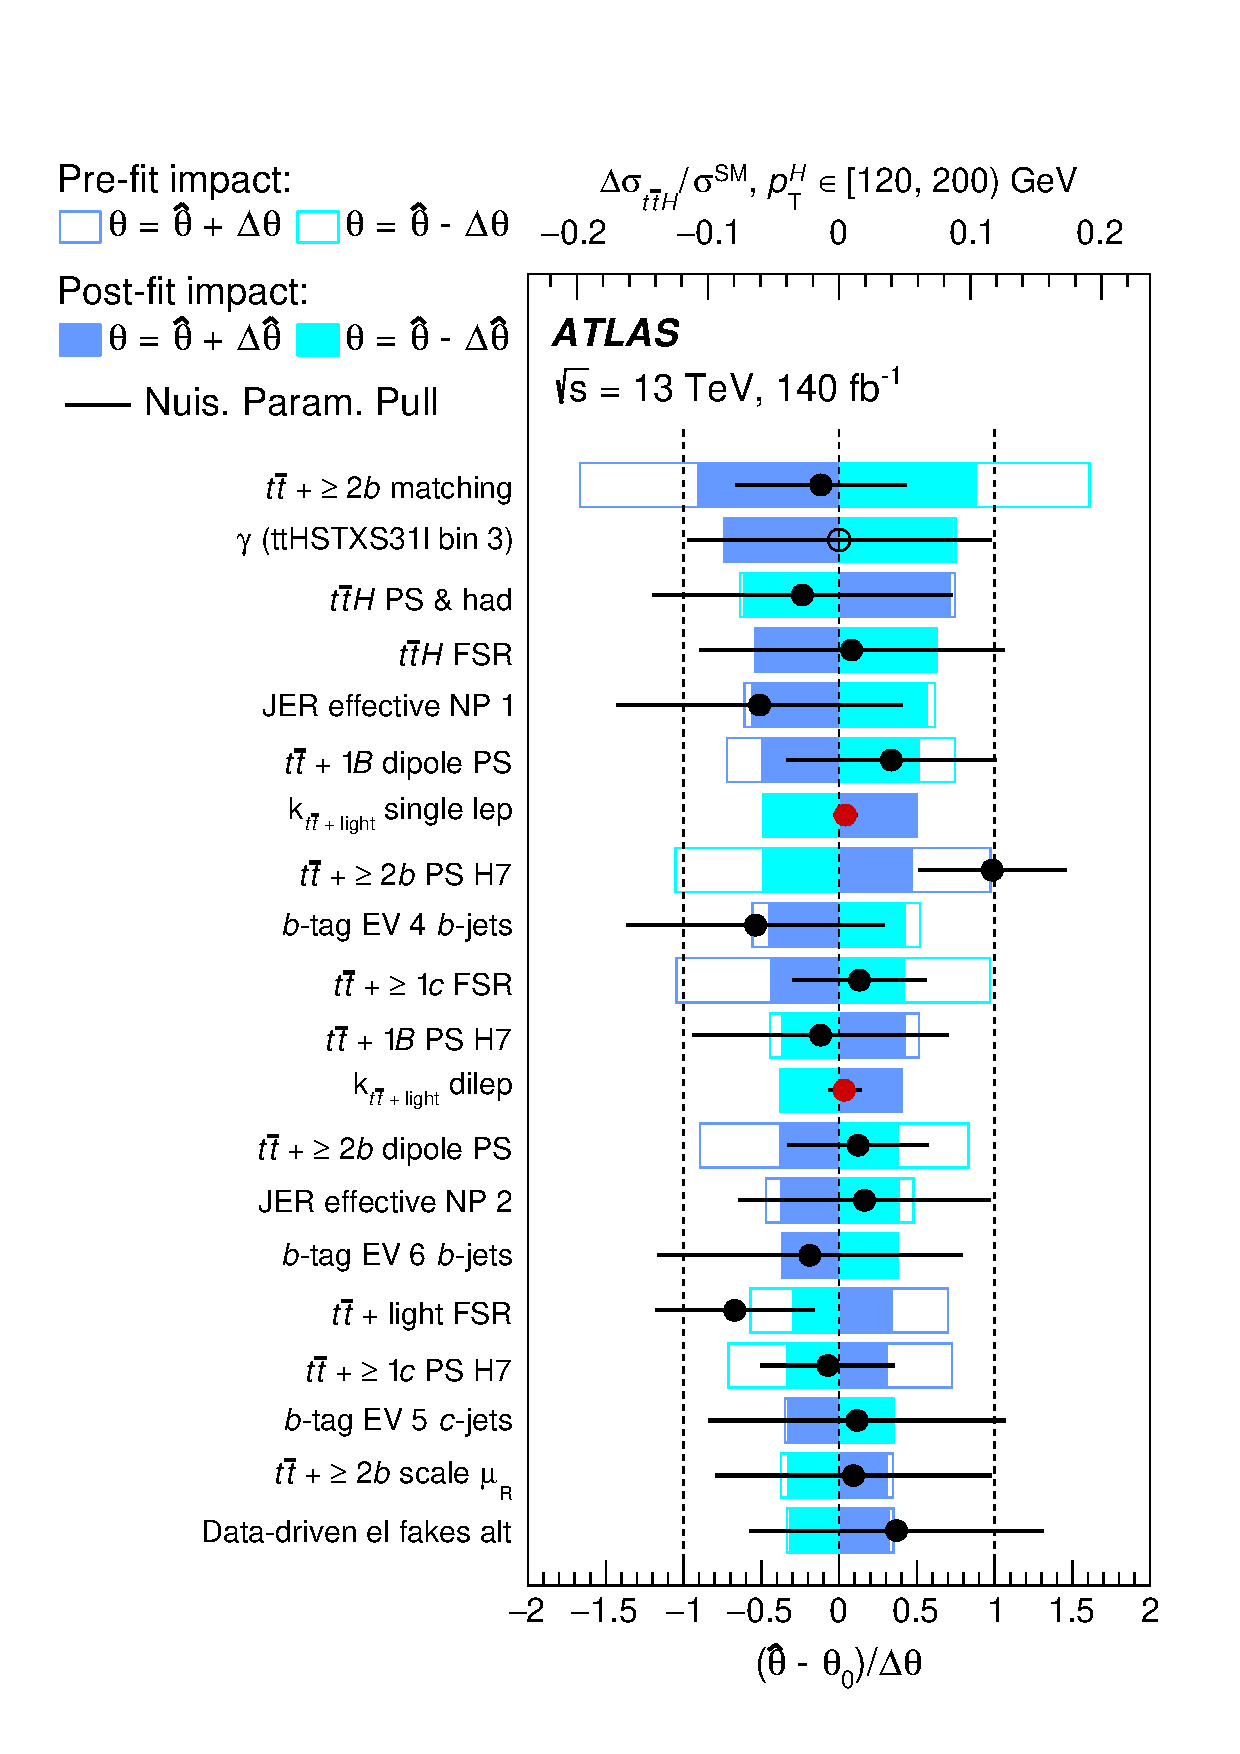
\includegraphics[width=\linewidth]{Section_tthbb_analysis/figures/Results/Ranking_ttH_ptH_120_200.pdf}
        \caption{}
    \end{subfigure}
    
    \vspace{0.5cm} % space between rows
    
    % Row 2: 3 images
    \begin{subfigure}{0.3\textwidth}
        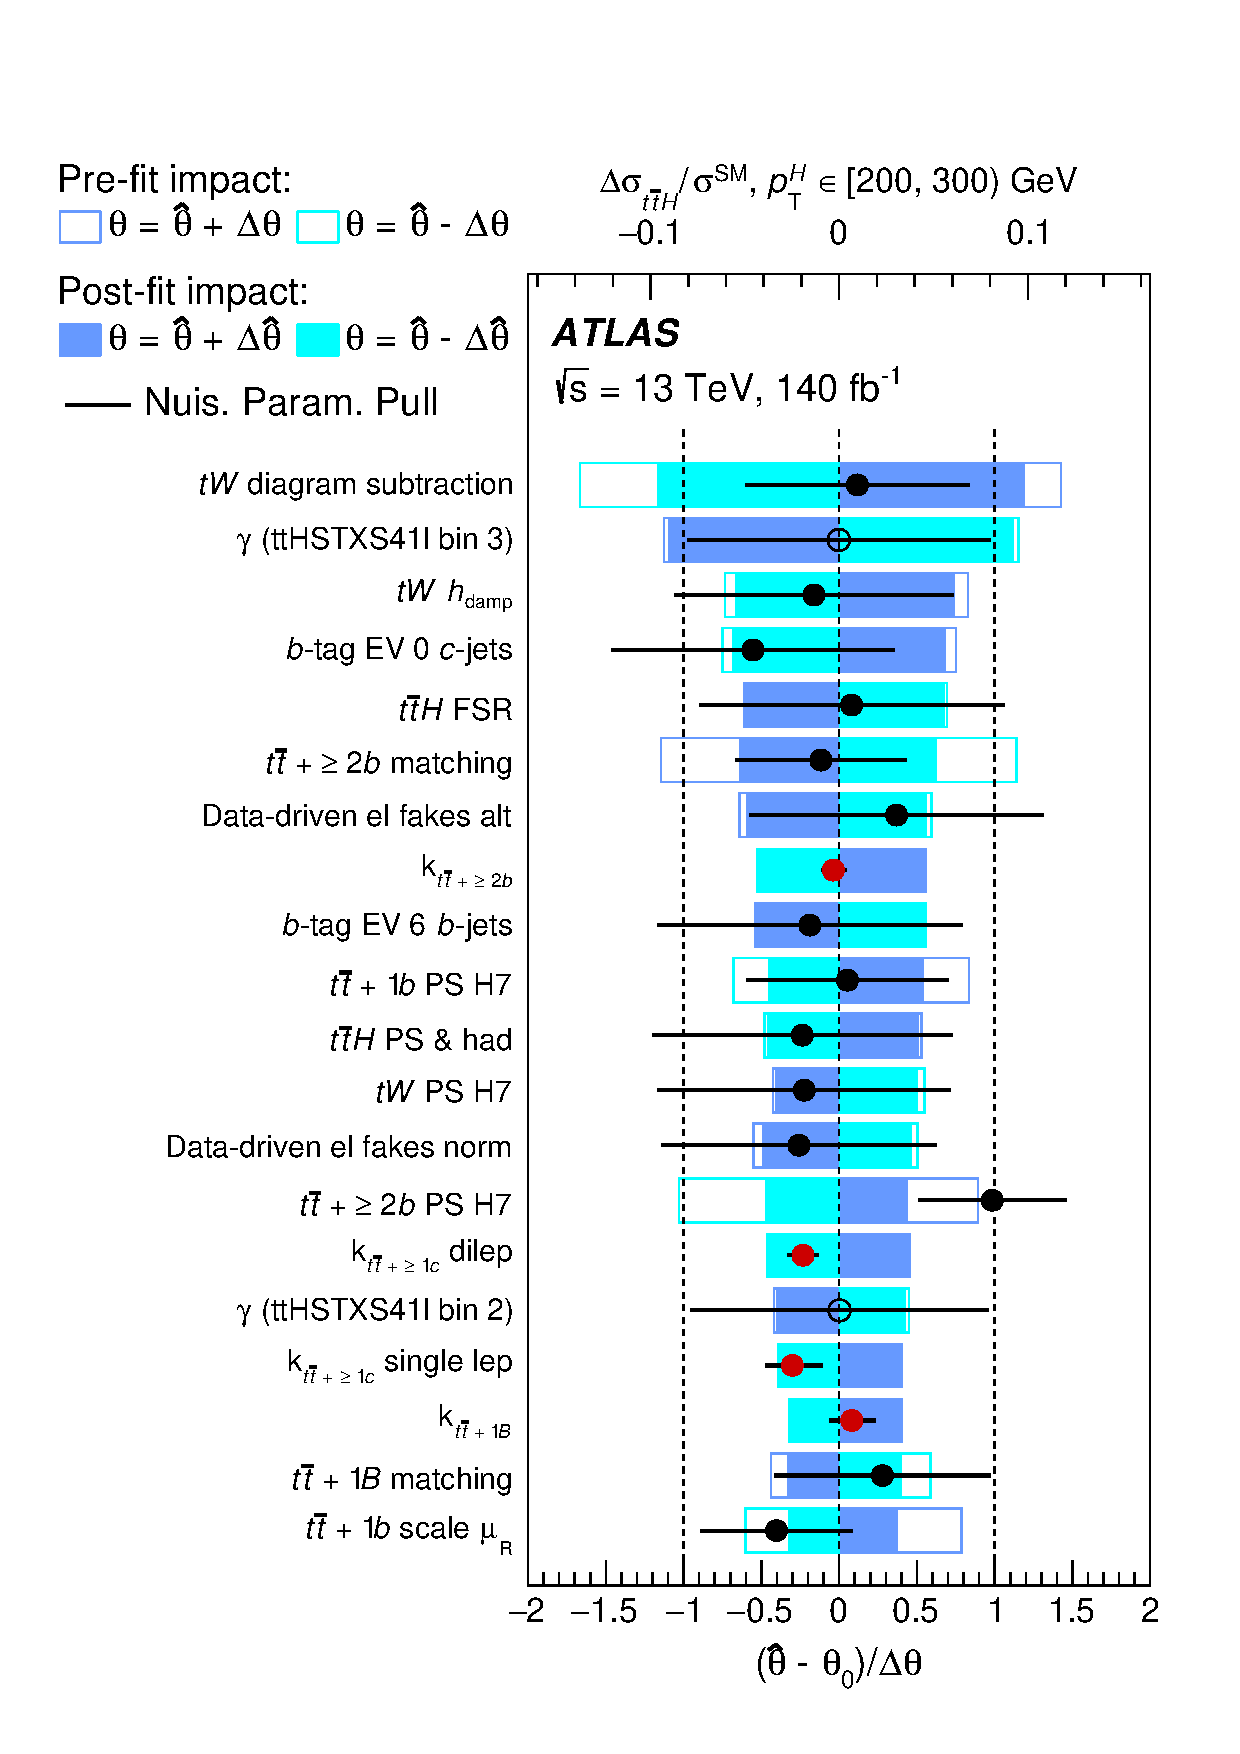
\includegraphics[width=\linewidth]{Section_tthbb_analysis/figures/Results/Ranking_ttH_ptH_200_300.pdf}
        \caption{j}
    \end{subfigure}
    \hfill
    \begin{subfigure}{0.3\textwidth}
        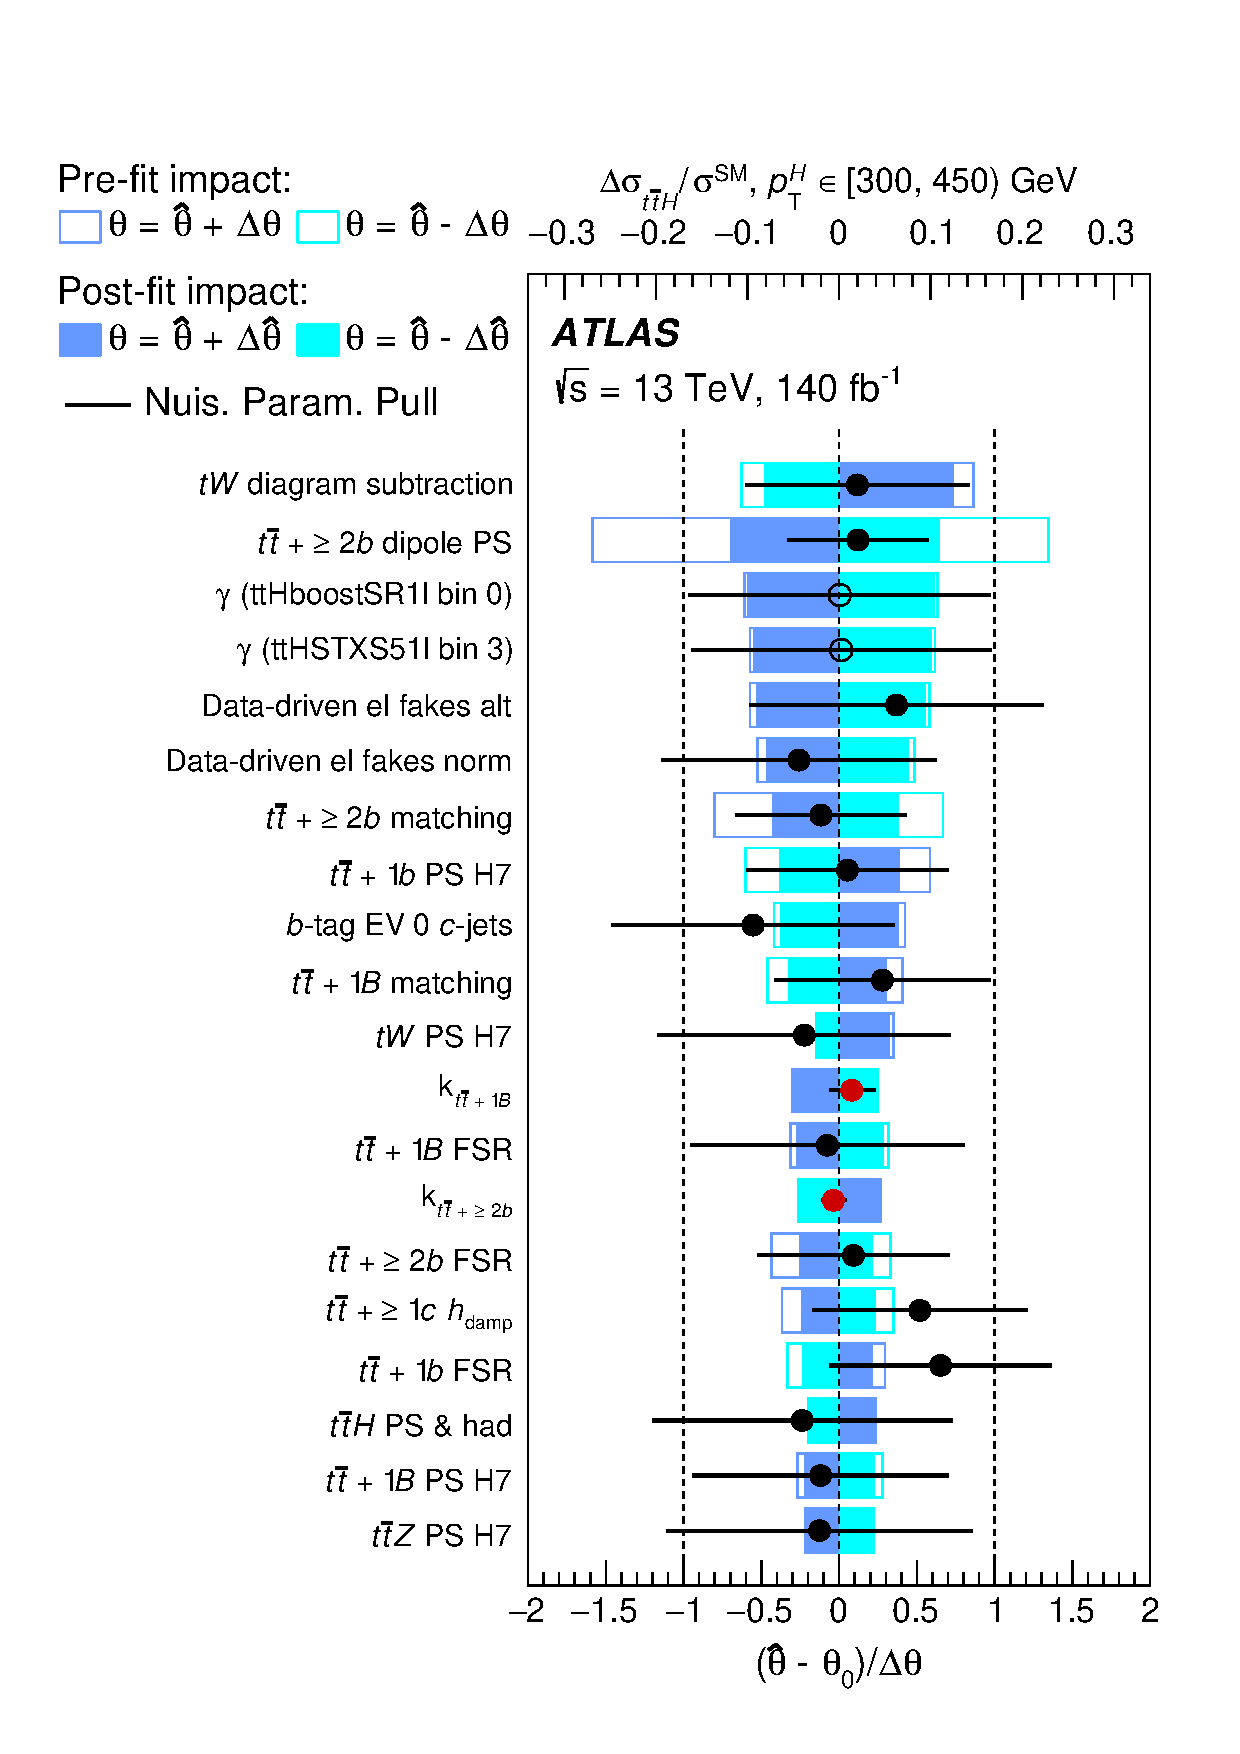
\includegraphics[width=\linewidth]{Section_tthbb_analysis/figures/Results/Ranking_ttH_ptH_300_450.pdf}
        \caption{}
    \end{subfigure}
    \hfill
    \begin{subfigure}{0.3\textwidth}
        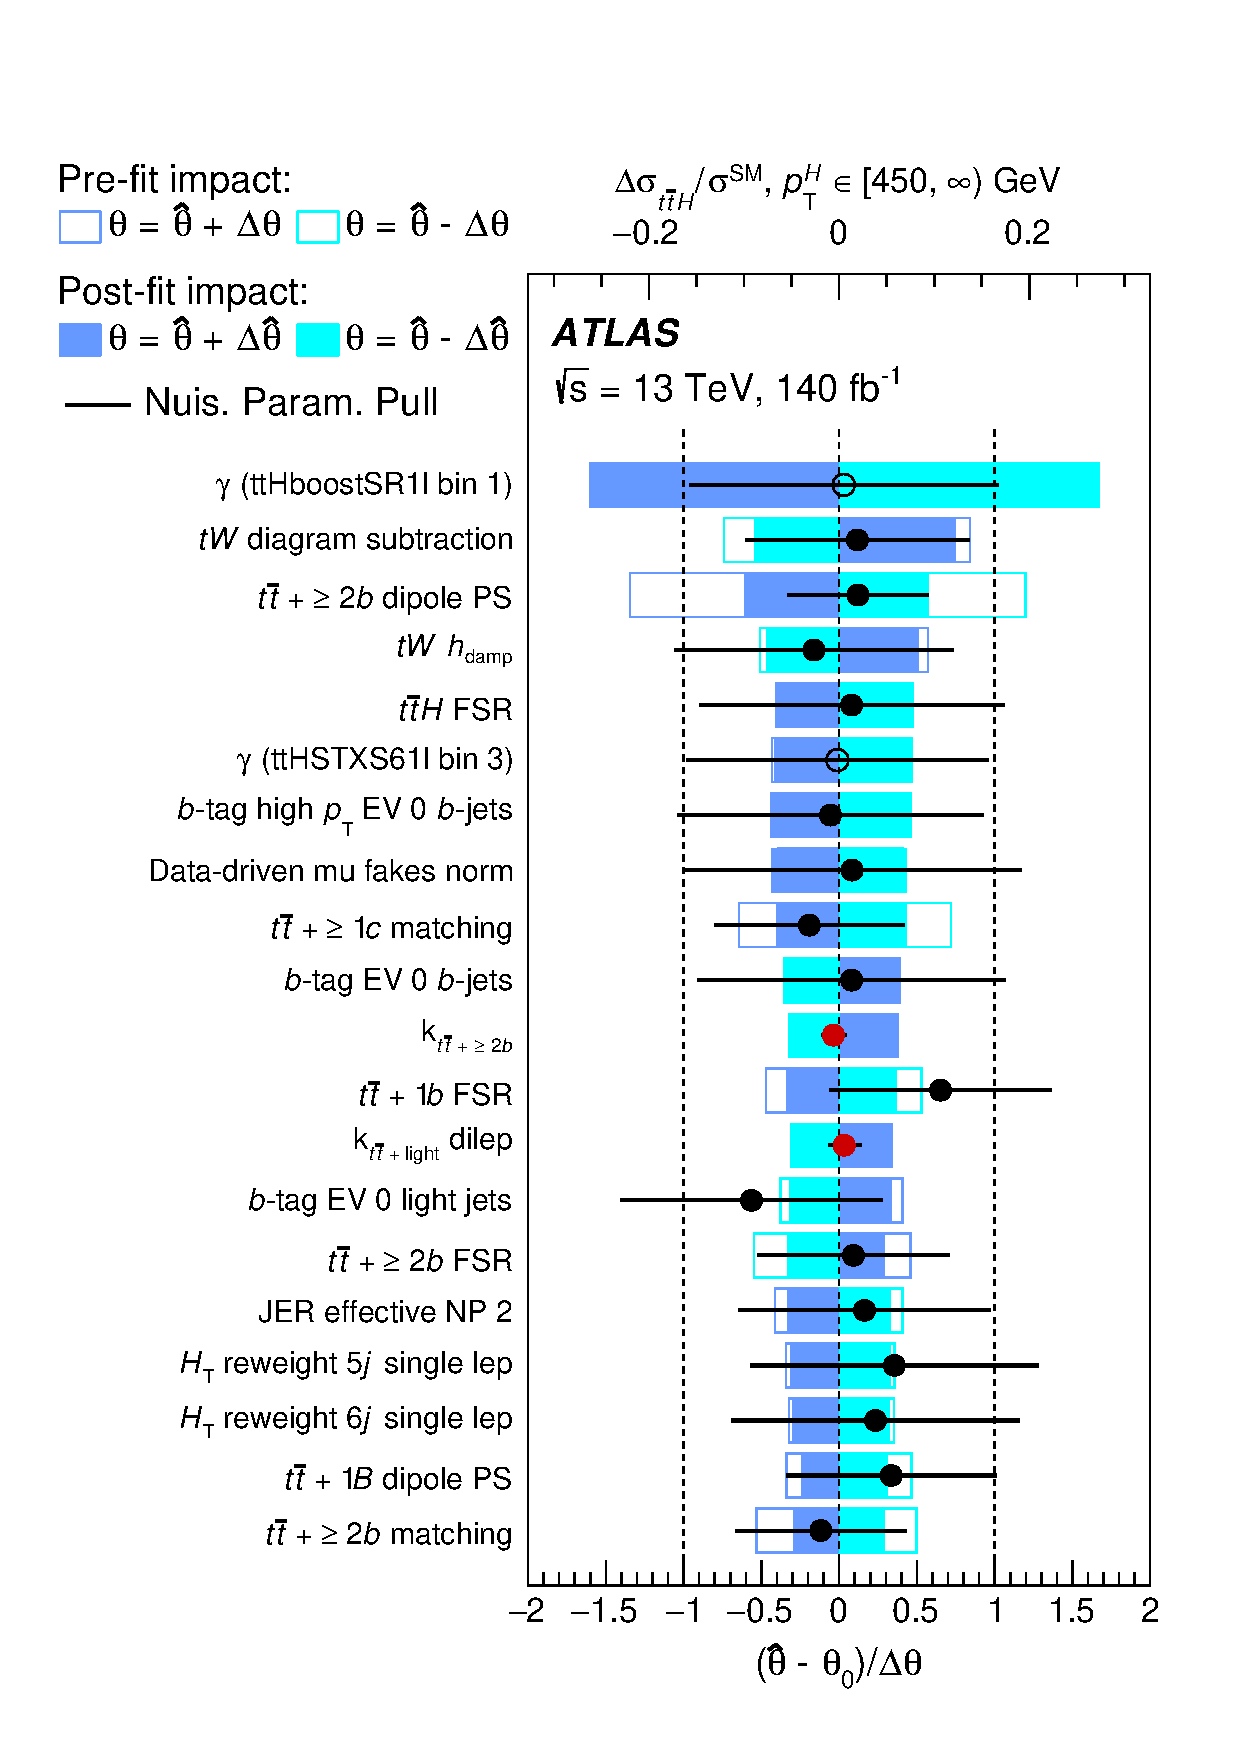
\includegraphics[width=\linewidth]{Section_tthbb_analysis/figures/Results/Ranking_ttH_ptH_gt450.pdf}
        \caption{}
    \end{subfigure}

    
\caption{Ranking of the 20 modelling and experimental systematic uncertainties with the largest post-fit impact in the inclusive STXS regions:  
(a) STXS 1,  
(b) STXS 2,  
(c) STXS 3,  
(d) STXS 4,  
(e) STXS 5,  
(f) STXS 6.}
    \label{fig:ranking_stxs}
\end{figure}
%% Big appendixes should be split off into separate files, just like chapters
%\input{app-myreallybigappendix}
